\documentclass[11pt,a4paper]{report}
\usepackage{subcaption} % supfigure requirement 

\usepackage[utf8]{inputenc}
\usepackage[T1]{fontenc}
\usepackage{amsmath}
\usepackage{amsfonts}
\usepackage{amssymb}
\usepackage{graphicx}
\usepackage{titlesec}
% setcounter is used so that subsubsections are included in the numbering scheme
%\setcounter{tocdepth}{4}
%\setcounter{secnumdepth}{4}
%% From: https://tex.stackexchange.com/questions/419662/change-style-of-chapter-headings-in-report-class-document
% Set margins
\usepackage[margin=3.0cm]{geometry}
\titleformat{\chapter}[hang]
{\normalfont\huge\bfseries}
{\thechapter}{20pt}{\huge}
\author{Espen Jettestuen \and Olav Aursj\o}
\title{BADChIMP manual}

\begin{document}
\maketitle


\tableofcontents

\chapter{Executive summary}
\label{sec:executive summary}
This code is developed for modeling fluid flow on the pore scale. The code can handle general geometries, non-Newtonian fluid rheologies and multi-phase systems. The code has been developed with the goal of providing a flexible environment for trying out new methods and add new physics.   

The code is in active development so we will suggested to download it from our github repository\footnote{You can access it from the following link https://github.com/eje74/BADChIMP-cpp} to get the most updated version. 


There are three major parts in this manual. Chapter \ref{sec:introduction and background}, \textbf{Introduction and background}, presents the theory behind the lattice Boltzmann method and should be a good short overview for students and researchers that want to understand the basics of the method. If you already are acquainted with he lattice Boltzmann method you could easily skip this section, although it can be useful to browse through it to get to know our notation. Chapter \ref{sec:code description and manual}, \textbf{Code description and manual}, describes the essential parts of the code and goes through a case study line by line. Chapter \ref{sec:simulation of non-Newtonian rheologies}, \textbf{Simulation of non-Newtonian rheologies}, describes how to simulate non-Newtonian rheologies using generalized expression for strain-rate-dependent viscosity.  


\chapter{Introduction and background}
\label{sec:introduction and background}
\section{The Lattice Boltzmann method}
\label{sec:the lattice boltzmann method}
The lattice Boltzmann method~\cite{kruger_lattice_2017, rothman1997lattice, sukop_lattice_nodate, succi_lattice_2001} is historically a generalization of the lattice gas methods for fluid flow. Later, it was shown that it was a discretization of the Boltzmann equation. It is the latter derivation that have gained traction in the lattice Boltzmann community and we will just sketch out how LB is related to the Boltzmann equation.

\subsection{Boltzmann equation}
\label{sec:boltzmann equation}
The Boltzmann equation~\cite{chapman_mathematical_1990} is given as
\begin{equation}
\partial_tf + c_i\partial_if = \Omega,
\end{equation}
where $f(t, \vec{x},\vec{c})$ is the single-particle distribution function, $\vec{c}$ is the microscopic particle velocity, and with a collision term $\Omega$ which is a function of the distribution functions. We will also use the notation that $\partial_t$ is the partial differential operator with respect to time, $t$ and $\partial_i$ is the partial differential operator with respect to the $i$'th Caretesian spatial coordinate, $x_i$. We also note that we will use Einsteins summation convention for repeated Cartesian indices.

The  equilibrium distribution for $f$ is given by the Maxwell-Boltzmann distribution
\begin{equation}
f^\mathrm{MB}(\vec{ c},\rho,\vec{u}) = \frac{\rho}{(2\pi c_s^2)^{3/2}}\exp\left(-\frac{|\vec{ c}-\vec{u}|^2}{2c_s^2}\right),
\end{equation}
where $c_s$ is the sound velocity, and $\rho$ and $\vec{u}$ are the macroscopic density and velocity, respectively. In lattice Boltzmann simulations, this is usually the BGK-collision term~\cite{bhatnagar_model_1954}
\begin{equation}
\Omega = -\frac{1}{\tau}\left(f-f^\mathrm{MB}\right).
\end{equation}
The macroscopic quantities are defined through different moments of the distribution function,
\begin{equation}
\begin{array}{lll}
\rho = \int f\,\mathrm{d}\vec{ c}, & \rho\vec{u} = \int \vec{ c} f\,\mathrm{d}\vec{ c}, & \rho\theta = \frac{1}{3}\int |\vec{ c}-\vec{u}|^2 f\,\mathrm{d}\vec{ c}.
\end{array}
\end{equation}
A standard notation for the moment of the distribution of microscopic velocities is 
\begin{equation}
\Pi_{i_1\dots i_n} = \int  c_{i_1}\cdots c_{i_n}f\,\mathrm{d}\vec{ c}.
\end{equation}



\subsection{Macroscopic equations}
\label{sec:macroscopic equations}
The macroscopic equations are derived from the Boltzmann equation by integration over different moments of the microscopic particle velocity coordinates. We will just illustrate the derivations using an example without any body force terms. Here we will use the integral notation $\int\,\mathrm{d}^3\vec{ c} $ as short-hand for $\int\,\mathrm{d} c_x\mathrm{d} c_y\mathrm{d} c_z$. The mass conservation law follows directly from the definition in the previous section: 
\begin{align*}
&\int \left(\partial_tf +  c_i\partial_if\right)\,\mathrm{d}^3\vec{ c} = \int \Omega\,\mathrm{d}^3\vec{ c} = 0 \\
&\partial_t\int f\,\mathrm{d}^3\vec{ c} + \partial_i\int c_i f\,\mathrm{d}^3\vec{ c} = 0 \\
&\partial_t\rho + \partial_i\rho u_i  = 0.
\end{align*}
The equations for impulse conservation are given by
\begin{align*}
&\int \left(c_i\partial_tf + c_ic_j\partial_j\right)\,\mathrm{d}^3\vec{c} = \int c_i\Omega\,\mathrm{d}^3\vec{c} = 0 \\
&\partial_t\int c_if\,\mathrm{d}^3\vec{c} + \partial_j\int c_i c_j f\,\mathrm{d}^3\vec{ c} = 0 \\
&\partial_t\rho u_i + \partial_j\Pi_{ij} = 0.
\end{align*}
Here, we obtain a second order tensor $\Pi_{ij}$ that we need to determine, which can be accomplished using the Chapman-Enskog expansion described in section \ref{sec:chapman-enskog expansion}. 

\subsection{The lattice Boltzmann numerical scheme}  
The procedure used to to derive the lattice Boltzmann equation from the Boltzmann equation is quite elaborate, so we will only give an executive sketch of the method with references to work that will supply the details.

The derivation can is conducted in two steps. First, the continuum of microscopic velocities is discretizied, so that we are left with an equation for a finite set of velocity distributions, $f_\alpha$, needed to described the systems. Here, $\alpha$ is just an integer denoting which microscopic velocity distribution it represents. After this first step we are left with a coupled system of differential equations. One for each microscopic velocity, that needs to be integrated in time. The second step is to discretize this integration.

For the first step we need to rewrite and Taylor expand $f^\mathrm{MB}$ in terms of $(u/c_s)$, i.e., the low Mach number limit, 
\begin{align*}
f^\mathrm{MB}(|\vec{u}-\vec{c}|) &= \frac{\rho}{(2\pi c_s^2)^{3/2}}\exp\left({-\frac{(\vec{u}-\vec{c})^2}{2c_s^2}}\right) = \frac{\rho \exp\left({-\frac{c^2}{2c_s^2}}\right)}{(2\pi c_s^2)^{3/2}}\exp\left({-\frac{u^2 -2\vec{c}\cdot\vec{u}}{2c_s^2}}\right) \\
&= \rho w(c)\left(1 + \frac{\vec{c}\cdot\vec{u}}{c_s^2} + \frac{(\vec{c}\cdot\vec{u})^2 - c_s^2u^2}{2c_s^4}\right) + \mathcal{O}\left((u/c_s)^3\right),
\end{align*}
where
\begin{equation*}
w(c) = (2\pi c_s^2)^{-3/2}\exp\left({-\frac{c^2}{2c_s^2}}\right).
\end{equation*}
It is this truncated expansion that is used for the equilibrium distribution in the lattice Boltzmann simulation. To derive the equilibrium values, one may now use this truncated expression to obtain the macroscopic variables. Abe~\cite{abe_derivation_1997}, and He and Luo~\cite{he_priori_1997,he_theory_1997}, described that, by using Gaussian quadrature, they could rewrite the integrals over $\vec{c}$, using sums over a finite sets of microscopic velocities that gave the same lattice structure as the standard lattice Boltzmann models\footnote{They had a different approach for handling the time integration. This turned out to be a sub-optimal solution.}. We can see this for ourselves by writing out the expression for the equilibrium moments 
\begin{equation}
\Pi_{i_1\dots i_n} = \int  c_{i_1}\cdots c_{i_n}f\,\mathrm{d}\vec{ c} \approx \int  \rho w(c)c_{i_1}\cdots c_{i_n}
\left(1 + \frac{\vec{c}\cdot\vec{u}}{c_s^2} + \frac{(\vec{c}\cdot\vec{u})^2 - c_s^2u^2}{2c_s^4}\right)
\,\mathrm{d}^3\vec{ c}.
\end{equation}     
Here, we can write the integral using a polynomial $P_{i_1\dots i_n}(\vec{c})$ in $\vec{c}$, and use Gaussian quadrature to obtain
\begin{equation}
\int  \rho w(c)P_{i_1\dots i_n}(\vec{c})\,\mathrm{d}\vec{ c} = \sum_\alpha \rho w_\alpha P_{i_1\dots i_n}(\vec{c}_\alpha),
\end{equation}
where $\alpha$ is an index used to identify the microscopic velocities used in the Gaussian quadrature and $w_\alpha = w(c_\alpha)$.  We only need a finite number of $f$-distributions to calculate the integrals. Hence, we do only need to know the evolution of the set of distribution, $f_\alpha$, used in the Gaussian quadrature scheme. And, from this, we are left with the set of differential equations,
\begin{equation}\label{eq:descrite boltzmann equation}
\partial_tf_\alpha + c_{\alpha i}\partial_if_\alpha = \Omega_\alpha,
\end{equation} 
where $\Omega_\alpha = -1/\tau(f_\alpha - f^\mathrm{MB}_\alpha)$. We also note that the Gaussion quadrature also supply us with the discrete equilibrium distribution 
\begin{equation}\label{eq:lb equilibrium distrubution}
f_\alpha^\mathrm{eq} = w_\alpha\left(1 + \frac{c_{\alpha i}u_i}{c_s^2} + \frac{Q_{\alpha ij}u_iu_j}{2c_s^4}\right),
\end{equation} 
where
\begin{equation}
Q_{\alpha ij} = c_{\alpha i}c_{\alpha j} - c_s^2\delta_{ij}.
\end{equation}
This is the standard expression used for the equilibrium distribution in LB models.This concludes the first step of the derivation of the LB method.

To begin our second step in the derivation, we note that the left hand side of the discrete Boltzmann equation, Eq.~\eqref{eq:descrite boltzmann equation}, is a 'free streaming' with velocity $c_\alpha$. Thus, by integration along this velocity direction over the time interval $\Delta t$  we get
\begin{align*}
f_\alpha(t + \Delta t, \vec{x} + &\Delta t\vec{c}_\alpha) - f_\alpha(t, \vec{x}) =\\
 &-\frac{\Delta t}{\tau}\int_0^{\Delta t}\left(f_\alpha(t + t^\prime, \vec{x} + t^\prime\vec{c}_\alpha) - f^\mathrm{MB}_\alpha(t + t^\prime, \vec{x} + t^\prime\vec{c}_\alpha) \right)\mathrm{d}t^\prime.
\end{align*} 
Using the trapezoidal rule on the right hand side, we obtain
\begin{align*}
&f_\alpha(t + \Delta t, \vec{x} + \Delta t\vec{c}_\alpha) - f_\alpha(t, \vec{x}) \approx\\
&-\frac{\Delta t}{\tau}\left(\frac{f_\alpha(t + \Delta t, \vec{x} + \Delta t\vec{c}_\alpha)-f^\mathrm{MB}_\alpha(t + \Delta t, \vec{x} + \Delta t\vec{c}_\alpha)}{2} + \frac{f_\alpha(t, \vec{x})-f^\mathrm{MB}_\alpha(t, \vec{x})}{2}\right), 
\end{align*} 
which is an approximation to the integral up to order $(\Delta t)^3$. In this expression, we have $f_\alpha(t + \Delta t, \vec{x} + \Delta t\vec{c}_\alpha)$ expressed using $f^\mathrm{MB}(t + \Delta t, \vec{x} + \Delta t\vec{c}_\alpha)$ which is an unknown quantity. To get around this problem, we make a change of variable from $f_\alpha$ to
\begin{equation}
f^*_\alpha(t, \vec{x}) = f_\alpha(t, \vec{x}) + \frac{\Delta t}{2\tau}\left(f_\alpha(t, \vec{x})-f^\mathrm{MB}_\alpha(t, \vec{x})\right),
\end{equation}
so that we end up with
\begin{equation}\label{eq:derived lb equation}
f^*_\alpha(t + \Delta t, \vec{x} + \Delta t\vec{c}_\alpha) - f^*_\alpha(t, \vec{x}) = -\frac{\Delta t}{\tau}\left(f^*_\alpha(t, \vec{x}) - f^\mathrm{MB}_\alpha(t, \vec{x}) \right).
\end{equation}
The reason why this works is that $\int \Omega\,\mathrm{d}^3c$ = $\int c_i\Omega\,\mathrm{d}^3c = 0$ for isolated systems, i.e., system without source terms. Hence, the redefinition of $f$ does not change the derived density and velocity of the isolated system, and we can find these variables using $f^*_\alpha$ instead of $f_\alpha$. We note that if we introduce mass sources and body forces we will need to add corrections to the collision terms. In the rest of this report, we will, through a renaming, denote $f_\alpha$ for $f^*_\alpha$. This concludes the second, and last, part of the derivation. Eq.~\eqref{eq:derived lb equation} is the equation known as \textit{the lattice Boltzmann equation}.

\subsection{Chapman-Enskog expansion}
\label{sec:chapman-enskog expansion}
The Chapman-Enskog expansion~\cite{chapman_mathematical_1990} is a method used to identify which macroscopic equations are modeled by the Boltzmann equation. This also includes how the parameters, describing the microscopic interactions, are related to the ones emerging on macroscopic scales. The Chapman-Enskog method is referred to as an asymptotic method so it is assumed to only show behavior in the long wavelength limit. We also note that the Chapman-Enskog expansion method does not tell us if the behavior, given by the Boltzmann equation, actually converges to the identified macroscopic equations.

The expansion is based on the assumption that both differential operators, $\partial_t$ and $\partial_i$, and distributions, $f$, can be expanded in terms that formally can be written as 
\begin{equation}\label{eq:epsilon partial_t}
\partial_t = \epsilon\partial^{(1)}_{t} + \epsilon^2\partial^{(2)}_{t} + \cdots,
\end{equation}
\begin{equation}\label{eq:epsilon partial_x}
\partial_i = \epsilon\partial^{(1)}_{i} + \epsilon^2\partial^{(2)}_{i} + \cdots,
\end{equation}
and
\begin{equation}\label{eq:epsilon f}
f = f^{(0)} + \epsilon f^{(1)} + \epsilon^2 f^{(2)} + \cdots.
\end{equation} 
The $\epsilon$ indicates the influence of the term in the long wavelength limit. Here, terms with higher powers of $\epsilon$ have less influence than those with lower powers of $\epsilon$.  The goal of the Chapman-Enskog expansion is to obtain the expression for the terms in the expansion of $f$, as function of the macroscopic variables. So that different moments of the microscopic velocities, for instance $\Pi_{ij}$, can be expressed as functions of the macroscopic variables and their partial derivatives. For the lattice Boltzmann method, it is common to apply this method to the discretize version of the the Boltzmann equation~\cite{kruger2017lattice, wolfram_cellular_1986}. 

We will use the LB equation, Eq.~\eqref{eq:derived lb equation}, as an example. The expansion on the left hand side is found by first applying a Taylor expansion to the left hand side of the LB equation
\begin{equation}
 f_\alpha(t + \Delta t, \vec{x} + \Delta t\vec{c}_\alpha)-f_\alpha(t, \vec{x}) = \sum_{n=1} \frac{(\Delta t)^n}{n!}\left((\partial_t + c_{\alpha i}\partial_i)^{n}f_\alpha\right)(t, \vec{x}).
\end{equation}   
The tedious part of the derivation is that we need to insert expressions Eqs.~\eqref{eq:epsilon partial_t}, \eqref{eq:epsilon partial_x}, and \eqref{eq:epsilon f} for $\partial_t$, $\partial_i$, and $f$, respectively, and then gather the terms with of the same power of $\epsilon$.  Here, we give these expressions for the three lowest levels of $\epsilon$'s
\begin{align*}
\mathcal{O}(\epsilon^0):& \ 0 \\
\mathcal{O}(\epsilon^1):& \left(\partial^{(1)}_{t} + c_{\alpha i}\partial^{(1)}_{i}\right)f_\alpha^{(0)} \\
\mathcal{O}(\epsilon^2):& \left(\partial^{(1)}_{t} + c_{\alpha i}\partial^{(1)}_{i}\right)f_\alpha^{(1)} + \left(\partial^{(2)}_{t} + c_{\alpha i}\partial^{(2)}_{i}\right)f_\alpha^{(0)} 
+ \frac{1}{2}\left(\partial^{(1)}_{t} + c_{\alpha i}\partial^{(1)}_{i}\right)^2f_\alpha^{(0)}, 
\end{align*}
where we have put $\Delta t = 1$ to make them more readable. The right-hand side of the equation is simpler. First of all, we identify that $f_\alpha^\mathrm{eq} = f_\alpha^\mathrm{MB}$ (see Eq.~\eqref{eq:lb equilibrium distrubution}) and we get that
\begin{align*}
\mathcal{O}(\epsilon^0):&  f^{(0)}_\alpha - f_\alpha^\mathrm{eq} \\
\mathcal{O}(\epsilon^1):& -\frac{1}{\tau}f^{(1)}_\alpha \\
\mathcal{O}(\epsilon^2):& -\frac{1}{\tau}f^{(2)}_\alpha.
\end{align*}
From the $\mathcal{O}(\epsilon^0)$, we note that we can put $f^{(0)}_\alpha = f_\alpha^\mathrm{eq}$. The important thing to notice here is that $f_\alpha^\mathrm{eq}$ is a function of macroscopic variables. By matching the $\epsilon$ terms, we note that we can express $f_\alpha^{(1)}$, on the right-hand side, using only $f_\alpha^{(0)}$, on the left-hand side. This pattern is general, so that the $\mathcal{O}(\epsilon^n)$, we have that the right-hand side, consists of $f$'s up to order $n$, while the left-hand side only include $f$'s, up to order $(n-1)$. This shows that we can, in principle, derive expressions for $f$, up to any order in $\epsilon$, using only macroscopic values. Going through these steps, using the expressions up to and including $\mathcal{O}(\epsilon^2)$, we can derive the Navier-Stokes equation as presented in section \ref{sec:fluid flow}. 

One important expression, from the Chapman-Enskog expansion, used in deriving models for non-Newtonian flow is the relation between $f_\alpha^\mathrm{neq} = f_\alpha-f_\alpha^\mathrm{eq}$ and the strain rate tensor, $E_{ij}$,
\begin{equation}\label{eq:f_neq e_ij}
\tau^{-1}f_\alpha^\mathrm{neq} = -w_\alpha\left(\frac{Q_{\alpha ij}}{c_s^2} + \frac{P_{\alpha ijk}u_k}{c_s^4}\right)\rho E_{ij} -w_\alpha\left(\frac{c_{\alpha i}}{c_s^2} +\frac{Q_{\alpha ij}u_j}{c_s^4} + \frac{P_{\alpha ijk}u_ju_k}{2c_s^6}\right)F_i,
\end{equation}
where $P_{\alpha ijk} = c_{\alpha i}c_{\alpha j}c_{\alpha k} - c_s^2\left(c_{\alpha i}\delta_{jk} + c_{\alpha j}\delta_{ik} + c_{\alpha k}\delta_{ij}\right)$.

\subsection{Lattice structures}
\label{subsec:lattice structures}
There are many different lattice structures that can be used in lattice Boltzmann simulations~\cite{wolf-gladrow_lattice-gas_2004}. We will not list them here, but we will point out the requirements that they need to fulfill. 

First of all, the notation used to describe a lattice is on the form D$n$Q$m$ where $n$ is a number that tells you the number of spatial dimensions of the lattice and $m$ tells you the number of basis vectors, $\vec{c}_\alpha$. 

A basis vector needs the have the property that if you are at a node position $\vec{x}$ then $\vec{x} + \vec{c}_\alpha$ also needs to be a node position. Finally, the sets of basis vectors, $\vec{c}_\alpha$, and weights, $w_\alpha$, need to fulfill the following summation rules, also called symmetries, to be able to simulation Navier-Stokes, 
\begin{equation}
\begin{array}{ll}
	\sum_\alpha w_\alpha = 1, & \sum_\alpha w_\alpha c_{\alpha i} = 0 \\ 
	\sum_\alpha w_\alpha c_{\alpha i}c_{\alpha j} = C_2\delta_{ij}, & \sum_\alpha w_\alpha c_{\alpha i}c_{\alpha j}c_{\alpha k} = 0 \\ 
	\sum_\alpha w_\alpha c_{\alpha i}c_{\alpha j}c_{\alpha k}c_{\alpha l} = C_4\left(\delta_{ij}\delta_{kl} + \delta_{ik}\delta_{jl}+ \delta_{il}\delta_{jk}\right), & \sum_\alpha w_\alpha c_{\alpha i}c_{\alpha j}c_{\alpha k}c_{\alpha l}c_{\alpha m} = 0.
\end{array} 
\end{equation}

\subsection{A complete lattice Boltzmann scheme}
In this section, we will supply a complete lattice Boltzmann scheme, which later is implemented in section \ref{sec:running a navier-stokes simulation}. The equations being solved are given in section \ref{sec:fluid flow}. The scheme is given by Eq.~\eqref{eq:derived lb equation},
\begin{equation}
f_\alpha(t + 1, \vec{x} + \vec{c}_\alpha) - f_\alpha(t, \vec{x}) = \Omega_\alpha,
\end{equation} 
where we have set $\Delta t = 1$. Now, since the system described in section~\ref{sec:fluid flow} has both a mass source term, $q$, and a body force term, $\vec{F}$, we will need corrections to our collision term~\cite{aursjo_inclusion_2018}
\begin{equation}
\Omega_\alpha = -\frac{1}{\tau}\left(f_\alpha - f^\mathrm{eq}_\alpha\right) + \Delta\Omega_\alpha,
\end{equation}
where
\begin{equation}
\Delta\Omega_\alpha = w_\alpha\left(1-\frac{1}{2\tau}\right)\left(q + \frac{Q_{\alpha ij}u_iu_j}{2c_s^4}q + \frac{c_{\alpha i}F_i}{c_s^2} + \frac{Q_{\alpha ij}u_iF_j}{c_s^4}\right).
\end{equation}
We will also need to add subsequent corrections to the evaluation of the density, $\rho$, and velocity, $\vec{u}$,
\begin{align*}
\rho &= \sum_\alpha f_\alpha + \frac{1}{2}q \\
\rho u_i &= \sum_\alpha c_{\alpha i}f_\alpha + \frac{1}{2}F_i.
\end{align*}
Further, it can be shown, using the Chapman-Enskog expansion, that the pressure $p = c_s^2\rho$, and the kinematic viscosity $\nu = c_s^2(\tau - 1/2)$.

The standard method to implement the lattice Boltzmann equation is a two-step procedure, with a collision step and a propagation step. In the collision step, we calculate the value of the LB distribution, $\tilde{f}_\alpha$, which is copied to the neighboring node in the $\alpha$-direction,
\begin{equation}
\tilde{f}_\alpha(t, \vec{x}) = f_\alpha(t, \vec{x}) + \Omega_\alpha(t, \vec{x}). 
\end{equation}
In the propagation step\footnote{This can also be referred to as  a streaming step}, values are copied from one neighbor node to another, following the velocity basis, so that
\begin{equation}
f_\alpha(t+1, \vec{x}+\vec{c}_\alpha) = \tilde{f}_\alpha(t, \vec{x}).
\end{equation} 
If the system has solid walls, we will get situations where the right-hand side of the above equation is not known, and we will need to supply a value using a boundary conditions. A standard method in LB models is to use a so-called bounce back scheme. The bounce back scheme that we use, in our standard case, is known as the half-way bounce back scheme. If we assume that we do not know the value of $\tilde{f}_\alpha(t, \vec{x}-\vec{c}_\alpha)$, as the node, at position $(\vec{x}-\vec{c}_\alpha)$, is inside the solid, the scheme says that we can use the value at $\vec{x}$ in the opposite direction of $\vec{c}_\alpha$, which we will call $\vec{c}_{\overline{\alpha}} = -\vec{c}_\alpha$. The propagation step then becomes
\begin{equation*}
f_\alpha(t+1, \vec{x}) = \tilde{f}_{\overline{\alpha}}(t, \vec{x}).
\end{equation*}  
This scheme will put a no-slip boundary condition on a wall located between positions $\vec{x}$ and $\vec{x}-\vec{c}_\alpha$.

\section{Continuum equations}
\label{sec:continuum_eqs}

\subsection{Fluid flow}
\label{sec:fluid flow}
The state of a moving fluid may be described through its velocity $\vec{u}(t,\vec{x})$, its pressure $p(t,\vec{x})$, and its mass density $\rho(t,\vec{x})$ at any position $\vec{x}$ and at any time $t$.
These quantities are governed by an equation of state, together with mass and momentum conservation. Using the Einstein summation convention, where Latin indices denote Cartesian
spatial components, mass and momentum conservation may, in component form, be described through \cite{batchelor2000introduction, landau87} 
\begin{align}
\partial_t \rho + \partial_i  (\rho u_i) &= q\, , \label{eq:cont_eq}
\\
\rho \left(\partial_t u_i + u_j \partial_j
u_i \right) &= - \partial_i p  + F_i + q u_i 
+ \partial_j \sigma'_{i j} -\partial_j T_{ij}\, , \label{eq:N-S_eq} 
\end{align}
where $q(t,\vec{x})$ is a mass source or sink, $p(t,\vec{x})$ is the pressure of the fluid, $F_i(t,\vec{x})$ is the
component of any applied volume force, $\sigma'_{ij}(t,\vec{x})$ are the components of the deviatoric stress tensor, and $T_{ij}$ are the components of any other stresses imposed on the fluid. For the fluid motion to be fully described, an additional equation of state is required to describe the relation between the pressure and the mass density of the fluid. 

\subsection{The deviatoric stress tensor $\sigma'_{i j}$}
\label{sec:the deviatoric stress tensor}
For Newtonian fluids, the relationship between the viscous stress and the strain rate
is per definition perfectly linear, and the viscosity is independent of the state of
motion or stress in the fluid. Here, the deviatoric stress tensor
\begin{align}
\sigma'_{i j} = \rho \nu \bigg[2E_{i j}
-\frac{2}{d} \partial_k u_k
\delta_{i j} \bigg] + \xi \partial_k u_k
\delta_{i j} \label{eq:viscStressTensor}
\end{align}
expresses the viscous stress tensor. Here, ${E_{i j} = (1/2)\big[\partial_i u_j + \partial_j u_i\big]}$
is the strain rate tensor, $\nu$ and $\xi$ are, respectively, the kinematic shear viscosity and the bulk (or volume) viscosity of the fluid, and $d$ is the number of spatial dimensions in the system. 


\subsection{Reactive Advection Diffusion}
We consider here, in addition, diffusion of a quantity $\varphi(t,\vec{x})$ influenced by the external fluid flow. This quantity is the concentration,
defined relative to the fluid density. It may be shown \cite{landau87} that, on component form, this process is described by the
equation
\begin{align}
\rho (\partial_t \varphi + u_i \partial_i \varphi) = \partial_i (D \rho \partial_i \varphi) + R - \varphi^k q,\label{eq:AD_eq}
\end{align}
where $D$ is the diffusivity and $R (t,\vec{x})$ is any given source term.
Such a source term could for instance arise from the change in concentration of a chemical component due to bulk chemical
reactions.



\chapter{Code description and manual} 
\label{sec:code description and manual}
\section{Installation and compilation}
\label{sec:Installation}

\subsection{Download}
The code is available from the github repository: 
\begin{verbatim}
	https://github.com/eje74/BADChIMP-cpp
\end{verbatim}
This repository can be cloned to your local machine using the following command line argument:
\begin{verbatim}
    $ git clone git@github.com:eje74/BADChIMP-cpp.git
\end{verbatim}
This assumes that the user has setup ssh to work with github. The BADChIMP code is then cloned into the folder \texttt{BADChIMP-cpp}.

\subsection{Compilation on linux} To compile the code, run the following command-line argument
\begin{verbatim}
    /BADChIMP-cpp$ ./make.sh <name_of_folder_with_main_file>
\end{verbatim}
in the code root folder, which is \texttt{BADChIMP-cpp} if you have followed the instruction above. The argument \texttt{<name{\_}of{\_}folder{\_}with{\_}main{\_}file>} tells in which folder the main-file to be complied is allocated. The standard case, \texttt{std{\_}case}, is build if no argument is given. The main-file folders are sub-folders in \texttt{BADChIMP-cpp/src}. This script will make a \texttt{build} folder, run \texttt{cmake} from that folder and then run \texttt{make}. 
This can also be done, by hand, using the following recipe: 
\begin{verbatim}
    /BADChIMP-cpp$ mkdir <build-folder-name>
    /BADChIMP-cpp$ cd <build-folder-name>
    /BADChIMP-cpp$ cmake -DLBMAIN:STRING="<name_of_folder_with_main_file>" ./..
    /BADChIMP-cpp$ make
\end{verbatim}

\subsection{Compilation on Windows} 
Make sure that open MPI is installed\footnote{See https://docs.microsoft.com/en-us/archive/blogs/windowshpc/how-to-compile-and-run-a-simple-ms-mpi-program. Download and run \texttt{msmpisetup.exe} and \texttt{msmpisdk.msi}.}  Install cmake for Windows.\footnote{See https://cmake.org/}. Run cmake from root directory to generate Visual Studio C++ project, or simply use VSCode.
\begin{table}
	\begin{tabular}{|l|l|}\hline
		Folder name & Description \\ \hline
		\texttt{std{\_}case} & Standard case, single fluid Navier-Stokes solver \\ \hline
		\texttt{two{\_}phase} & Two phase simulator \\ \hline
    \end{tabular}
	\caption{List of different main files}
\end{table}

\subsection{Making a new main folder}
In this sub section we will go through the steps to add a new main folder, which we will call \texttt{new{\_}main{\_}folder} in the following, to the code repository.

The first step is to make a new sub directory in the \texttt{./BADChIMMP/src/} directory, which we in this example has called \texttt{./BADChIMMP/src/new{\_}main{\_}folder}. Then copy the \texttt{main.cpp} and \texttt{CMakeLists.txt} from the \texttt{std{\_}case} folder. If you for some reason want to change the name of the main file in the new main folder, remember to also change the main file-name in \texttt{CMakeLists.txt}. This is the whole recipe for creating a new main folder. To generate a \texttt{build} folder just follow the instruction given in section \ref{sec:Installation} for running the \texttt{make.sh}-script.

\section{Structure of the main file}
\subsection{Main file outline}
Here is an executive overview of the main-file for a standard pore scale simulations. Each section is described in more detail on the following pages.
\begin{verbatim}
<include libraries>
<set lattice type>

int main()
{
  // SETUP
  <mpi>
  <input and output directories>
  <grid, geometry and mpi-communication>
  <read input-file>
  <macroscopic fields, i.e. density, velocity et c.>
  <boundary conditiones>
  <lattice Boltzmann velocity distributions>
  <vtk-output>
  
  // TIME LOOP
  for (int i = 0; i <= nIterations; i++) {
  	// NODE LOOP
    for (auto nodeNo: bulkNodes) {
      <calculate macroscopic values>
      <calculate collision term>
      <propagate>
    }
    <swap data>
    <mpi-communication>
    <apply bondary conditions>
    <write to file>
  }
  <end of program rutines>
}

\end{verbatim}
\subsection{Lattice type}
\begin{verbatim}
// SET THE LATTICE TYPE
#define LT D2Q9
\end{verbatim}
The lattice type is set as the macro \texttt{LT}. The lattice type is a name of a static class and are defined in header files in \texttt{BADChIMP-cpp/src/lbsolver}. The header files for the different lattice types are listed in \texttt{BADChIMP-cpp/src/LBSOLVER.h}.
The different lattice types are defined in separate head files with the naming convention \texttt{LBd<num dim>q<num dir>.h}. We note that in the current setup we have assumed that the last direction, that is, the direction with the larges index, is the rest direction. The naming convention for the static class is \texttt{D<num dim>Q<num dir>}. The lattice class contains a number of variables together with functions for performing simple manipulations based on the lattice structure. We will list most of them in the following tables.
 
The standard lattice structure constants are listed in table ~\ref{tab:basic lattice structure}, besides the number of spatial and lattice directions, this also includes different expressions involving the sound speed, $c_s$, which is defined in section \ref{subsec:lattice structures}. We will just note the notation $C_2=c_s^2$ and $C_4=c_s^4$.   
\begin{table}
	\centering
	\begin{tabular}{|c|l|}\hline
		Variable name & description \\ \hline
		\texttt{nD} & Number of spatial directions \\ 
		\texttt{nQ} & Number of lattice directions \\ \hline
		\texttt{c2} & $=C_2$ \\ 
		\texttt{c2Inv} & $=1/C_2$ \\ \hline
		\texttt{c4} & $=C_4$ \\ 
		\texttt{c4Inv} & $=1/C_4$ \\ 
		\texttt{c4Inv0{\_}5} & $=1/(2C_4)$ \\ \hline
	\end{tabular}
	\caption{Basic lattice structure}
	\label{tab:basic lattice structure}
\end{table}
Basis vectors and vector operations are defined using functions, but the weights, $w_\alpha$, and derived quantities are simple to access through standard vector notation, see table \ref{tab:lattice weights}.
\begin{table}
	\centering
	\begin{tabular}{|c|l|}\hline
		Variable name & description \\ \hline
		\texttt{w0} & rest particle weight \\ 
		\texttt{w1} & nearest neighbor weight \\ 
		\texttt{w2} & nest nearest neighbor weight \\ 
		\vdots & \vdots \\ \hline
		\texttt{w0c2Inv} & $=\texttt{w0}/C_2$ \\ 
		\texttt{w1c2Inv} & $=\texttt{w1}/C_2$ \\ 
		\texttt{w2c2Inv} & $=\texttt{w2}/C_2$ \\ 
		\vdots & \vdots \\ \hline
		\texttt{w[q]} & $=w_q$ where $0\leq q < \texttt{nQ}$ \\ \hline
	\end{tabular}
	\caption{Lattice weights}
	\label{tab:lattice weights}
\end{table}
The variables and functions to access the basis vectors are given in table \ref{tab:lattice basis vector}.
\begin{table}
	\centering
	\begin{tabular}{|c|l|}\hline
		Variable name & description \\ \hline
		\texttt{c(q, i)} & $=c_{qi}$ \\ 
		\texttt{reverseDirection(q)} & $\vec{c}_{\texttt{reverseDirection(q)}} = -\vec{c}_{q}$ \\ \hline 
		\texttt{cNorm[q]} & $=|\vec{c}_q|$ \\ \hline
	\end{tabular}
	\caption{Lattice basis vectors}
	\label{tab:lattice basis vector}
\end{table}

\begin{table}
	\centering
	\begin{tabular}{|c|l|}\hline
		Variable name & description \\ \hline
		\texttt{dot(u, v)} & $=\vec{u}\cdot\vec{v}$ \\ 
		\texttt{grad(s)} & $=\nabla s$ \\ \hline
		\texttt{cDot(q, u)} & $=\vec{c}_q\cdot\vec{u}$ \\ 
		\texttt{cDotAll(u)} & $=\{\vec{c}_q\cdot\vec{u}|\ 0\leq q < \texttt{nQ}\}$ \\ \hline
		\texttt{qSum(f(0, nodeNo))} & $=\sum_\alpha f_\alpha(t, \vec{x})$ \\
		\texttt{qSumC(f(0, nodeNo))} & $=\sum_\alpha \vec{c}_\alpha f_\alpha(t, \vec{x})$ \\ \hline
	\end{tabular}
	\caption{Functions used to work with vectors and distributions. More information is given in the text}
	\label{tab:vector and distribution functions}
\end{table}
The function for vector and distribution manipulations are listed in table \ref{tab:vector and distribution functions}. In general, all function in this table that takes vector like input will assume that the elements can be accessed using the \texttt{[$\cdots$]} notation. The functions that return vectors will return \texttt{std::valarray<lbBase\_t>} type objects.

Finally, we have the constants that relates to multi-phase simulations, where we have an set of constants that is needed for the Reis and Phillips~\cite{reis_lattice_2007} implementations of color gradient methods. The constants are listed in table \ref{tab:lattice weights two phase} and referrers to Equation. 28 in Reis and Phillips~\cite{reis_lattice_2007},
\begin{equation*}
\left(\Omega_q^k\right)^{(2)} = \frac{A_k}{2}|\vec{F}|\left[\frac{\left(\vec{F}\cdot\vec{c}_q\right)^2}{|\vec{F}|^2}- B_q\right].
\end{equation*}
\begin{table}
	\centering
	\begin{tabular}{|c|l|}\hline
		Variable name & description \\ \hline
		\texttt{B0} & rest particle weight \\ 
		\texttt{B1} & nearest neighbor weight \\ 
		\texttt{B2} & nest nearest neighbor weight \\ 
		\vdots & \vdots \\ \hline
		\texttt{B[q]} & $=B_q$ where $0\leq q < \texttt{nQ}$ \\ \hline
	\end{tabular}
	\caption{Lattice weights for the two phase color gradient method.}
	\label{tab:lattice weights two phase}
\end{table}

\subsection{mpi (setup)}
The lattice Boltzmann code uses the MPI (Message Passing Interface) library to handle parallel computation on clusters of cpu's. The standard setup code for the mpi is
\begin{verbatim}
// *********
// SETUP MPI
// *********
MPI_Init(NULL, NULL);
int nProcs;
MPI_Comm_size(MPI_COMM_WORLD, &nProcs);
int myRank;
MPI_Comm_rank(MPI_COMM_WORLD, &myRank);
\end{verbatim} 
The variables \texttt{nProcs} and \texttt{myRank} holds the total number of processors used in the computations and the rank of the current process, respectively.

\subsection{Input and output directories (setup)}
After initializing mpi we need to define the directory paths for input and output files. In BADChIMP there are two types of input files: one relating to geometry and geometry partitioning, and another which supplies the standard input variables.
\begin{verbatim}
// ********************************
// SETUP THE INPUT AND OUTPUT PATHS
// ********************************
std::string chimpDir = "/BADChIMP-cpp/";
std::string mpiDir = chimpDir + "input/mpi/";
std::string inputDir = chimpDir + "input/";
std::string outputDir = chimpDir + "output/";
\end{verbatim}
In the code above the base directory is saved in \texttt{chimpDir}. The code searches for the geometry related files in \texttt{mpiDir} while the standard input file is in directory \texttt{inputDir}. The output files from the simulations are written into \texttt{outputDir}.  

\subsection{Setup grid and geometry}
This section of the code creates the object that handles input from the user, sets up the system geometry, node partitioning and the mpi-communication protocol. 
The input data-file, with \texttt{input.dat} as default name, is read into an \texttt{Input} object, while the vtklb-geometry files are read by an \texttt{LBvtk}-object. The \text{grid}-object, that defines the neighborhood of nodes, depends on the \texttt{vtklb} object. The \texttt{Nodes}-object, that holds information about the node type (e.g., if it is fluid, wall etc.), depends on both the \texttt{grid} and \texttt{vtklb}-objects. And finally, the \texttt{BndMpi}, that handles the transfer of data between processor partition boundaries, is dependent on the \texttt{nodes}-, \texttt{grid}-, and \texttt{vtklb}-objects.  
\begin{verbatim}
// ***********************
// SETUP GRID AND GEOMETRY
// ***********************
Input input(inputDir + "input.dat");
LBvtk<LT> vtklb(mpiDir + "tmp" + std::to_string(myRank) + ".vtklb");
Grid<LT> grid(vtklb);
Nodes<LT> nodes(vtklb, grid);
BndMpi<LT> mpiBoundary(vtklb, nodes, grid);
\end{verbatim}
In the next sections we will go through the different objects that are declared here.

\subsection{Input}
\label{sec:input}
The \texttt{Input}-object expects an input file in a nested block structure, and uses \texttt{\#} for comments. A block is defined by two sets of angle brackets, the first pair contains a name (and possibly a type definition), and the second pair contains a \texttt{end} key word which ends the block.
\begin{verbatim}
<block-name>
  # bulk content
<end>
\end{verbatim}
Blocks can also be nested:
\begin{verbatim}
<block-nameA>
  # bulk content
  <block-nameB>
    # bulk content
  <end>
  # more bulk content
<end>
\end{verbatim}
So, how to we add values to be read by the program? Outside of an block structure one uses the \texttt{set} key-word on the form
\begin{verbatim}
set name value  # e.g. set pi 3.14
\end{verbatim}
In the program you access this value using the \texttt{input}-object
\begin{verbatim}
double var = input["name"];
\end{verbatim}
Inside an block a name followed by either one or a list of numerical vales:
\begin{verbatim}
<block-name>
  nameA value              # e.g. pi 3.14 
  nameB value1 value2 ...  # e.g. prime 2 3 5 7 
<end>
\end{verbatim}
These inputs are imported in the following manner,
\begin{verbatim}
double val = input["block-name"]["nameA"];
std::vector<int> valarr = input["block-name"]["nameB"]; 
// valarr = {2, 3, 4, 5, 7}
\end{verbatim} 
Nested blocks are accessed in a similar manner, by ordering the block names from left to right, where the left is the outermost block and the right is the innermost, e.g.,
\begin{verbatim}
<block-nameA>
  <block-nameB>
    pi 3.14
  <end>
<end>
\end{verbatim}
is read as
\begin{verbatim}
double pi = input["block-nameA"]["block-nameB"]["pi"];
\end{verbatim}
Values can also be added in matrix form
\begin{verbatim}
<name type>
 val(0,0)   val(0,1)   ... val(0,m-1)
 val(1,0)   val(1,1)   ... val(1,m-1)
  ...
 val(n-1,0) val(n-1,1) ... val(n-1,m-1) 
<end>
\end{verbatim}
Here, \texttt{type} can be \texttt{char} or \texttt{int}, or be omitted assuming that the entries are of floating point type. The matrix type is accessed as an vector, 
\begin{verbatim}
// valmat = {val(0,0), val(0,1), ... ,val(0,m-1), 
//           val(1,0), ...,val(n-1,m-1)}
std::vector<double> valmat = input["name"];
\end{verbatim}
When using a \texttt{char} type, the data is read digit by digit and no white-space characters should separate the values which now should be a numerical digit (0-9), e.g.,
\begin{verbatim}
<binary char>   
  0101
  1110
<end>
\end{verbatim}
and is read as
\begin{verbatim}
std::vector<int> binary = input["binary"]; 
// binary = {0,1,0,1,1,1,1,0} 
\end{verbatim}   

\subsection{LBvtk}\label{sec:lbvtk}
The \texttt{LBvtk} object reads the vtklb geometry files together with any appended data. You can use this object to get access to appended data\footnote{For now we have only implemented functionality for obtaining scalar attributes.}. To get access to the scalar attribute we need to use the class methods \texttt{toAttribute} and \texttt{getScalarAttribute} to access the data and to get the range of nodes number from \texttt{beginNodeNo} and \texttt{endNodeNo}. As an example we will show how to read the attribute \texttt{"name"} of \texttt{double}-type from file and print it to screen,
\begin{verbatim}
vtklb.toAttribute("name");
for (int n=vtklb.beginNodeNo(); n<vtklb.endNodeNo(); ++n) {
    std::cout << vtklb.getScalarAttribute<double>() << std::endl;
}
\end{verbatim}
Here, \texttt{toAttribute(std::string s)} takes the attribute name as a string input. \texttt{beginNodeNo()} return the first node number read and \texttt{endNodeNo()} gives the end range of node numbers. \texttt{getScalarAttribute<type>()} reads entries of numerical type \texttt{type} which is given as a template typename.

\subsection{Grid}
\label{sec:grid}
The \texttt{Grid} object contains information about which nodes are part of a node's neighborhood and the spatial position of each node. Information about the neighborhood of a node is found by using the \texttt{neighborhood}-function,
\begin{verbatim}
auto neighbor_node = grid.neighbor(alpha, node); 
// return the node number of the 
// neighboring node in the alpha 
// direction

auto neighbor_nodes = grid.neighbor(node);  
// Returns a list of the node numbers
// to all nodes in the neighborhood                                            
\end{verbatim}
The position in Cartesian coordinates is found by using \texttt{pos},
\begin{verbatim}
auto pos = grid.pos(node); 
// pos = x_pos, y_pos, z_pos

auto pos_i = grid.pos(node, index); 
// return the node's position's 
// Cartesian index  
\end{verbatim} 
To find a node number from a position array, you can use \texttt{Grid}'s \texttt{nodeNo}:
\begin{verbatim}
int node = 10;
auto pos = grid.pos(node);
int node_from_pos = grid.nodeNo(pos); 
// node_from_pos = 10
\end{verbatim}
The \texttt{getNodePos} returns the position of nodes in Cartesian coordinates as an integer vector on the from $[x, y, z]$. The function is overloaded. So, given a list of node numbers, the syntax is 
\begin{verbatim}
std::vector<int> list_of_nodes = {2, 4, 6};
auto list_of_pos = grid.getNodePos(list_of_nodes);
// list_of_pos is of type std::vector<std::vector<int>>
// If 
// pos_of_node2 = {1, 1, 2}
// pos_of_node4 = {3, 1, 5}
// pos_of_node6 = {2, 5, 2}
// then
// list_of_pos = {{1, 1, 2}, 
//                {3, 1, 5},  
//                {2, 5, 2}}
\end{verbatim}
The function can also be used with \textit{two} arguments: a begin node and an end node number. The function will then return the position as a vector starting with the begin node and ending with the end node. The end node's position is not part of the output vector. An example is given below:  
\begin{verbatim}
int begin_node = 2;
int end_node = 4;
auto list_of_pos = grid.getNodePos(begin_node, end_node);
// list_of_pos = {pos_node2, pos_node3}
\end{verbatim}
Finally, to get the total number of node numbers represented in grid we can use \texttt{grid.size()}. Note that this includes the potential default ghost node label.
\begin{verbatim}
auto total_number_node_labels = grid.size();
\end{verbatim}

\subsection{Nodes}
\label{sec:nodes}
\begin{figure}
	\centering
	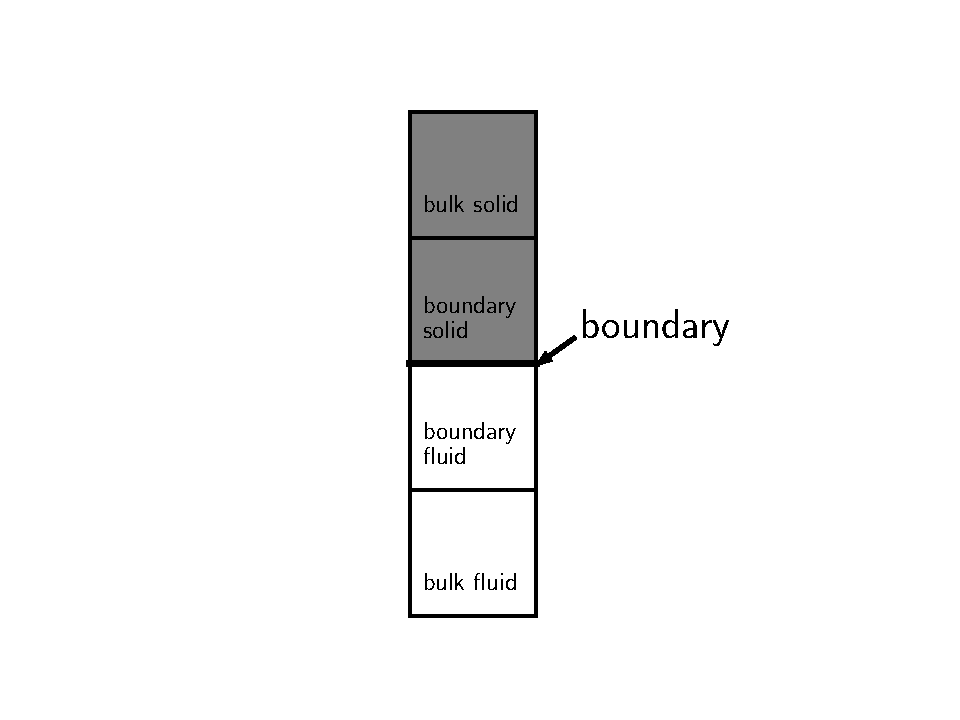
\includegraphics[width=0.7\linewidth]{Figures/nodetypes.pdf}
	\caption{A sketch of the different node types. In this figure gray shows the solid part of the geometry and with is the fluid. The thick black line is the solid fluid boundary.}
	\label{fig:nodetypes}
\end{figure}
The \texttt{Nodes} object contains more information about the nodes. Nodes comes in five different types, as far as the \texttt{Nodes}-class is concerned: the default ghost node, solid nodes of bulk and boundary type, and fluid nodes of bulk and boundary type (see Fig.~\ref{fig:nodetypes}). A fluid node is a boundary node if it has a solid node in its neighborhood, and vice versa for solid nodes. The fluid node is a bulk node if it is not at boundary node. The reason for this labeling is that a boundary node will have unknown LB distributions after the streaming step, as, at least, one velocity distribution comes from a solid node. Besides the solid and fluid nodes, we can have a default ghost node that is used as a dummy node. The default ghost node is treated as a solid node. Each node type is given a numerical value, as presented in Table \ref{tab:node type value}.
\begin{table}
	\centering
	\begin{tabular}{|l|r|}\hline
		{\bf Node type} & {\bf value} \\ \hline
		default ghost & -1 \\ \hline
		solid bulk & 0 \\ \hline
		solid boundary & 1 \\ \hline
		fluid boundary & 2 \\ \hline
		fluid bulk & 3 \\ \hline
	\end{tabular}
	\caption{Numerical key value for representing node types}
	\label{tab:node type value}
\end{table}
The node type value is accessed using the \texttt{getType} function. The code below prints the node type value for all nodes in the grid-object  
%\samepage{
\begin{verbatim}
for (int n=0; n < grid.size(); ++n) 
{
    std::cout << "Node number " << n << " ";
    std::cout << "has the node type value " << nodes.getType(n);
    // nodes.getType(n) returns an int
    std::cout << std::endl;
}
\end{verbatim}
%}
The \texttt{nodes} object also contains many Boolean functions, returning true/false values for the question "is node ... of type ...": 
\begin{verbatim}
int node_number = 4;
 
nodes.isDefault(node_number); 
// return true of the node is a default ghost node, false otherwise

nodes.isBulkSolid(node_number); 
// return true of the node is a bulk solid node, false otherwise

nodes.isSolidBoundary(node_number); 
// return true of the node is a solid boundary node, false otherwise

nodes.isFluidBoundary(node_number); 
// return true of the node is a fluid boundary node, false otherwise

nodes.isBulkFluid(node_number); 
// return true of the node is a bulk fluid node, false otherwise
\end{verbatim}
We can also ask the \texttt{nodes} object if a node is fluid or solid. A fluid node is a node that is either a fluid boundary or a bulk fluid, whereas a solid is either a solid boundary, a solid bulk or a default ghost. The class functions used for this is 
\begin{verbatim}
nodes.isSolid(node_number); 
// return true of the node is a solid node, false otherwise

nodes.isFluid(node_number); 
// return true of the node is a fluid node, false otherwise
\end{verbatim}
The \texttt{nodes} object also holds some information about the parallel partitioning of the system. Spesifically, it holds the information about which processor rank a node represents. Typically, a node that is a bulk fluid node on one processor will be a boundary fluid node on one of its neighboring processors, as it will need to get velocity distributions that are calculated on the former processor. More information about how the code handles parallelization is found in sections ~\ref{sec:parallelization} and ~\ref{sec:geometry file format}. 
To obtain which processor rank a node represents we can use 
\begin{verbatim}
auto node_rank = nodes.getRank(node_number);
// node_rank is set to an int containg the rank number given by mpi
\end{verbatim}
To find out if the rank of a node is the same as the rank of the current process use 
\begin{verbatim}
auto true_false = nodes.isMyRank(node_number);
// True if the node has the same rank as the current process, false otherwise
\end{verbatim}
Finally you could ask if it is an mpi boundary node with 
\begin{verbatim}
auto true_false = nodes.isMpiBoundary(node_number);
// True if node is an mpi boundary, false otherwise
\end{verbatim}

\subsection{BndMpi}
\label{sec:bndmpi}
The \texttt{BndMpi} class holds algorithms for transferring information between processors in a parallel setup. Most of this is done "under the 
hood" in the constructor when the \texttt{mpiBoundary} object is declared, but we need to specify in the code when we want this communication, between processors, to occur. The \texttt{BndMpi} class contains methods for the communication of scalar fields and velocity distribution fields. The scalar field communication is invoked by the overloaded class method \texttt{communciateScalarField}: 
\begin{verbatim}
ScalarField rho(2, grid.size());

mpiBoundary.communciateScalarField(0, rho);
// communicates rho's 0'th field to the neighboring processors

mpiBoundary.communciateScalarField(1, rho);
// communicates rho's 1'th field to the neighboring processors

mpiBoundary.communciateScalarField(rho);
// communicates all rho's fields to the neighboring processors
// In the case above this is the same as
// mpiBoundary.communciateScalarField(0, rho);
// mpiBoundary.communciateScalarField(1, rho);
\end{verbatim}
The \texttt{ScalarField} class is discussed later in this section. The communication of velocity distribution fields are similar to that of the scalar fields:
\begin{verbatim}
LbField<D2Q9> f(2, grid.size());

mpiBoundary.communicateLbField(0, f, grid);
// communicates f's 0'th field to the neighboring processors

mpiBoundary.communicateLbField(1, f, grid);
// communicates f's 1'th field to the neighboring processors

mpiBoundary.communicateLbField(f, grid);
// communicates all rho's fields to the neighboring processors
\end{verbatim}
The \texttt{LbField} class is discussed later in this section.

\subsection{Boundary and bulk nodes}
\label{sec:boundary and bulk nodes}
There are several functions that can be used to partition the nodes in the different groups: \texttt{findBulkNodes}, \texttt{findSolidBndNodes}, \texttt{findFluidBndNodes}.
The \texttt{findBulkNodes} returns a list of bulk node labels, where a bulk node is assumed to be a fluid node that is on the current processor. This function is defined to return the nodes that are part of the standard LB algorithm. The function is overloaded:
\begin{verbatim}
auto bulkNodes = findBulkNodes(nodes);
// returns a stl int vector with node numbers and 
// takes a Nodes-object as input

std::vector<int> marker;
...
auto bulkNodesMarker = findBulkNodes(nodes, marker);
// returns a stl int vector with node numbers, and 
// takes a Nodes-object and an stl int vector as input.
// Besides the above mentioned criteria, a bulk node
// will also need to be marked with a zero in the 
// maker vector. 
\end{verbatim}
The \texttt{findSolidBndNodes} returns a list of node numbers for the solid boundaries nodes on the given processor. The function is not overloaded:  
\begin{verbatim}
auto solidBoundaryNodes = findSolidBndNodes(nodes);
// returns a std int vector with node numbers and 
// takes a Nodes-object as input
\end{verbatim}
The \texttt{findFluidBndNodes} also returns a list of node numbers of fluid boundary nodes, but in the same way as \texttt{findBulkNodes} it is overloaded allowing for the addition of a marker vector:
\begin{verbatim}
auto fluidboundarNodes = findFluidBndNodes(nodes);
// returns a stl int vector with node numbers and 
// takes a Nodes-object as input

std::vector<int> marker;
...
auto fluidboundarNodesMarker = findFluidBndNodes(nodes, marker);
// returns a stl int vector with node numbers, and 
// takes a Nodes-object and an stl int vector as input.
// Besides the above mentioned criteria, a bulk node
// will also need to be marked with a zero in the 
// maker vector. 
\end{verbatim}

\subsection{Boundary conditions}

The boundary conditions are usually based on the \texttt{Boundary} class. The boundary class contains a list of  boundary nodes where the all basis directions are categorized in $\gamma$, $\beta$, or $\delta$. 
But first, we will expand a bit on the classification of nodes. As noted before, we call a node solid if that node does not stream a value. Hence, if a neighbor node is a solid, the distribution propagated from that node will be treated as unknown. A solid node will not alway be a solid part of the geometry. For instance, the ghost node neighbors of inlet and outlet boundaries will be treated as solids in the \texttt{Node} class. This will be used in the \texttt{Boundary} constructor which uses \texttt{Nodes}' \texttt{isSolid} to decide if a node is a solid or not.

The classification of boundary node directions is based on directions pairs. A pair is defined as a lattice direction and its reverse. As mentioned, there are three types of link pairs $\beta$, $\gamma$, or $\delta$, which
are characterized according to whether or not the values are known after streaming. That is, are values streamed from fluid nodes (known) or
from solid nodes (unknown)? The categorization of links are given in Table~\ref{tab:categorization of links}, and illustrated in figure \ref{fig:boundary distribtuion categoris}. 
\begin{table}
	\centering
	\begin{tabular}{|c|l|}\hline
		{\bf direction} &  \\ \hline
		$\vec{c}_\beta$ & unknown \\ 
		$-\vec{c}_\beta$ & known \\ \hline
		$\vec{c}_\gamma$ & known \\ 
		$-\vec{c}_\gamma$ & known \\ \hline
		$\vec{c}_\delta$ & unknown \\ 
		$-\vec{c}_\delta$ & unknown \\ \hline
	\end{tabular}
	\caption{link categories}
	\label{tab:categorization of links}
\end{table}
In a \texttt{Boundary} object just one direction for each link is recorded. So, to get all directions we need to use the \texttt{revDir} function of the recorded directions to obtain both directions in the pair.
Firstly, the \texttt{Boundary} class contains a function to get access to the boundary nodes:
\begin{figure}[h]
	\centering
	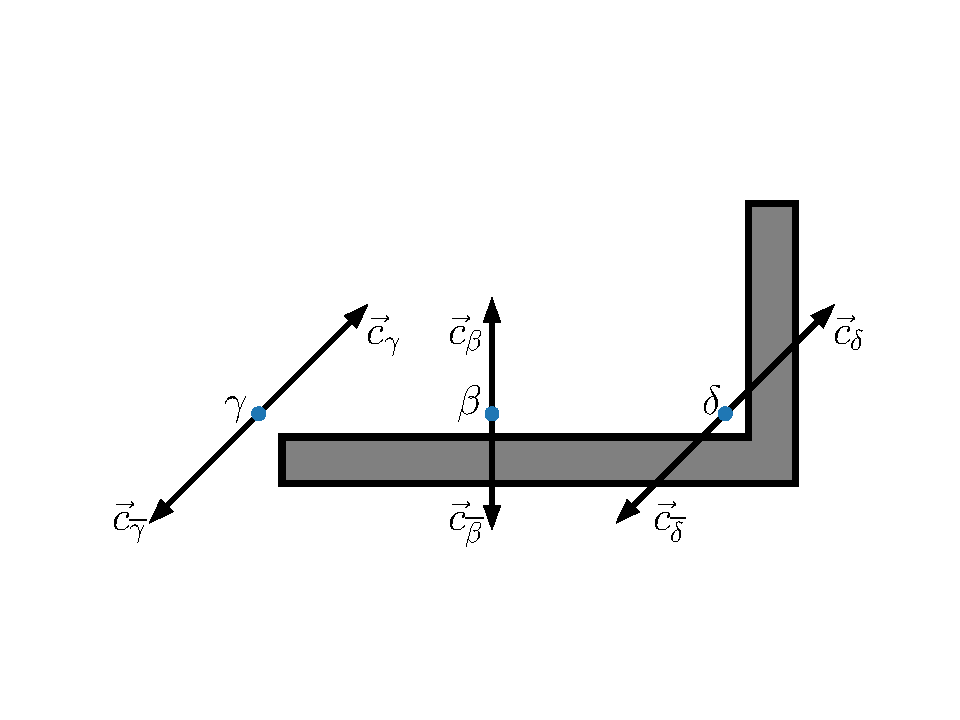
\includegraphics[width=0.7\linewidth]{Figures/laplace_boundary_condition.pdf}
	\caption{The figure shows the three categories of boundary links, $\gamma$, $\beta$ and $\delta$ to the left, middle and right, respectively. Here, we have denoted the revere direction by using an overline-symbol over the Greek-letter label.}
	\label{fig:boundary distribtuion categoris}
\end{figure}
\begin{verbatim}
std::vector<int> list_of_boundary_nodes;
...
// Constructor
Boundary<D2Q9> boundary(list_of_boundary_nodes, nodes, grid);

// Boundary node list
auto number_of_boundary_nodes = boundary.size();
// Holds the length of the list of boundary nodes

int boundaryNumber; 
...
auto nodeNumber = boundary.nodeNo(boundaryNumber);
// nodeNumber holds the node number of the boundaryNumber-element in the 
// list of boundary nodes.
\end{verbatim}
Secondly, the \texttt{Boundary} class contains a function to obtain the number of pairs in the given categories, and list them. To find the number of links of a given type, at a given boundary node, we can use the following functions:
\begin{verbatim}
auto number_of_beta_links_inline = boundary.nBeta(boundaryNumber);
// Returns the number of beta links

auto number_of_gamma_links_inline = boundary.nGamma(boundaryNumber);
// Returns the number of gamma links

auto number_of_delta_links_inline = boundary.nDelta(boundaryNumber);
// Returns the number of delta links
\end{verbatim}
We note that each link consist of a pair of directions. So, to obtain the total number of directions, we will need to multiply each number-of-links variable by 2. To find the list of links contained in each category, we can use the functions listed below. We note that each element in the list returned contains only one of the directions in a link pair. For the $\gamma$ and $\delta$ directions, we know that both directions are either known or unknown, respectively. But, for the $\beta$ direction we have specified that the direction returned is the unknown direction.
\begin{verbatim}
std::vector<int> list_of_beta_directios = boundary.beta(boundaryNumber);
// list of the unknown direction member from each beta link pair for bondary
// member element boundaryNumber

std::vector<int> list_of_gamma_directios = boundary.gamma(boundaryNumber);
// list of one direction member from each gamma link pair for bondary member
// element boundaryNumber

std::vector<int> list_of_delta_directios = boundary.delta(boundaryNumber);
// list of one direction member from each delta link pair for bondary member
// element boundaryNumber
\end{verbatim}
Finally we have added the function \texttt{dirRev} to find the reverse direction of lattice direction:
\begin{verbatim}
int dir;
... // dir will hold an arbitrary lattice direction
auto reverse_dir = boundary.dirRev(dir);
// reverse_dir holds the reverser direction of dir.
\end{verbatim}
To show the full use of the \texttt{Boundary} class, we will give an example of going through all boundary nodes in the \texttt{boundary} object and list all directions classified by link-type, and know and unknown values:
\begin{verbatim}
for (int n = 0; n < boundary.size(); n++) 
{
    int node = boundary.nodeNo(n); // Get node number
    std::cout << "Node number " << node << std::endl;
    // Print all beta values
    std::cout << "beta =";
    auto beta = boundary.beta(n);
    for (int q = 0; q < boundary.nBeta(n); ++q) {
        std::cout << " " << beta[q] << "(Unknown)";
        std::cout << " " << boundary.revDir( beta[n] ) << "(Known)";
    }
    std::cout << std::endl;
    // Print all gamma values
    std::cout << "gamma =";
    auto gamma = boundary.gamma(n); 
    for (int q = 0; q < boundary.nGamma(n); ++q) {
       std::cout << " " << gamma[q] << "(Known)";
       std::cout << " " << boundary.revDir( gamma[q] ) << "(Known)";
    }
    std::cout << std::endl;
    // Print all delta values
    std::cout << "delta =";
    auto delta = boundary.delta(n);
    for (int q = 0; q < boundary.nDelta(n); ++q) {
       std::cout << " " << delta[n] << "(Unknown)";
       std::cout << " " << boundary.revDir( delta[n] ) << "(Unknown)";
    }
    std::cout << std::endl;
}
\end{verbatim} 
\emph{Caution}: Note that a node number and the numbering of an element in the boundary node list are usually not the same number. We get the node number from the index of the boundary list by using the \texttt{nodeNo} function.

The class \texttt{HalfWayBounceBack} is used to enforce the half-way bounce-back boundary condition.  The declaration of an object of this class needs a list of nodes, a \texttt{Nodes} object, and a \texttt{Grid} object:
\begin{verbatim}
auto list_of_fluid_nodes = findFluidBndNodes(nodes);
// std vecter of node numbers of the nodes that are part of the boundary

HalfWayBounceBack<D2Q9> boundaryCondition(list_of_fluid_nodes, nodes, grid);
// Declaration of the a HalfWayBounceBack object. Besides the 
// list-of-fluid-nodes it takes a Nodes object and a Grids object as input.
\end{verbatim}
For a fluid simulations, we would expect the list-of-boundary-nodes to be fluid boundary nodes. We would also assume that the solid boundary nodes are part of the system, as this will hold the bounce back part of the distributions. The half-way bounce-back is effectively a part of the propagation routine. The conceptual picture is that the distributions hits a wall, located half way between the origin node and the destination node, where it is flipped and returns to the origin as the distribution going in the opposite direction as it left. This means that it could, and should, be applied straight after the bulk node loop. The boundary condition is applied using the overloaded \texttt{apply} class function:
\begin{verbatim}
LbField<D2Q9> f(2, grid.size());
// f holds two LB distributions

boundaryCondition.apply(0, f, grid);
// Applies the half-way bounce back to field 0

boundaryCondition.apply(1, f, grid);
// Applies the half-way bounce back to field 1

boundaryCondition.apply(f, grid);
// Applies the half way bounce back to all fields represented by f
// It is equivalent to running the two functions above, in this case 
\end{verbatim}

\subsection{Field classes}
\label{sec:field classes}
There are currently three field classes in BAChIMP: \texttt{ScalarField}, \texttt{VectorField}, and \texttt{LbField}: These represent fields of scalars, vectors, and LB distributions, respectively. The scalar and vector field objects are used to hold the fluid density and velocity, for instance. Below we see a standard initialization step in a LB simulation, where all densities are set to 1 and all velocities are set to 0.
\begin{verbatim}
// ******************
// MACROSCOPIC FIELDS
// ******************
// LT is a constant representing a lattice type
//
// Density
ScalarField rho(1, grid.size());
// Velocity
VectorField<LT> vel(1, grid.size());
// Initiate values
for (auto nodeNo: bulkNodes) {
    rho(0, nodeNo) = 1.0;
    for (int d=0; d < LT::nD; ++d)
        vel(0, d, nodeNo) = 0.0;
}
\end{verbatim}
The \texttt{ScalarField} object declaration, \texttt{ScalarField rho(1, grid.size())},  takes two input arguments. The first is the number of fields and the second is the size of the system. In the case here, we have only one field, and the number of elements matches the size of the system. The same input arguments are needed by the \texttt{VectorField<LT>} object. We also note that a vector field is a template class. We obtain the values from a scalar object by referring to the field and node number, so that
\begin{verbatim}
auto value = rho(0, 4);
// value has the type given by lbBase_t.
\end{verbatim}    
returns the value of the node with node number 4 in the 0'th field. We note that, as is standard in C++, we begin the numbering of fields with 0. There are two way to obtain values from a \texttt{VectorField} object:
\begin{verbatim}
auto value = vel(0, 1, 4);
// Return the value of component 1 at node number 4

auto vector = vel(0, 4);
// returns a std::valarray of lbBase_t elments 
// represnting the vector value at node number 4
\end{verbatim}
The number of components of a vector in a \texttt{VectorField} object is the same as the dimension of the lattice type. To set values we use the same notation as above for the \texttt{ScalarField} and for components of vectors for the \texttt{VectorField}, but if you want to assign a vector to a node use \texttt{VectorField}'s \texttt{set} function:
\begin{verbatim}
VectorField<LT> vector(1, 1);
VectorField<LT> vectorField(1, 10);
...
vectorField.set(0, 4) = vector(0, 0);
// Sets the vector at node 4 equal the value of vector(0, 0);  
\end{verbatim}
\texttt{ScalarField} and \texttt{VectorField} objects can be written to file and read using the class functions \texttt{writeToFile} and \texttt{readFromFile} using the syntax shown below.
\begin{verbatim}
ScalarField rhoWrite(2, grid.size());
...
std::string filename = "myfile";
rhoWrite.writeToFile(filename); // Write field to file

ScalarField rhoRead(2, grid.size());
rhoRead.readFromFile(filename); // Read from file
\end{verbatim}
The syntax is exactly the same for \texttt{VectorField} objects. Note that number of fields, number of nodes and, in the case for vector objects, spatial dimension must be the same for the written and read field objects.

The \texttt{LbField} class is similar to the \texttt{VectorField} class, except that the distribution is represented as a vector with the same number of elements as the number of basis vectors. Below we show how to initialize the distribution, $f_\alpha = w_\alpha\rho$,
\begin{verbatim}
// ***********************
// LB FIELD INITIALIZATION
// ***********************
LbField<LT> f(1, grid.size());  // LBfield
for (auto nodeNo: bulkNodes) {
    for (int q = 0; q < LT::nQ; ++q) {
        f(0, q, nodeNo) = LT::w[q]*rho(0, nodeNo);
    }
}
\end{verbatim} 
The declaration of a \texttt{LbField} object is equal to the declartion of a \texttt{VectorField} object, where the first argument is the number of fields and the second is the number of nodes.
As for vector fields, you access the element in a \texttt{LbField} object using the field number and node number to obtain a vector, containing all distribution values at a node. Or, one can specify field number, direction and node number to access a given direction at a node:
\begin{verbatim}
auto value = f(0, 7, 2);
// Return the value of the distribution component 7 
// at node number 2

auto distribution = f(0, 2);
// returns a std::valarray of lbBase_t elments 
// represnting the distribution value at 
// node number 4
\end{verbatim}
For the propagation step, $f_\alpha(t+1, \vec{x} + \vec{c}_\alpha) = \tilde{f}_\alpha(t,\vec{x})$, we can use a loop over all lattice directions
\begin{verbatim}
LbField<LT> f(1, grid.size());
LbField<LT> f_tilde(1, grid.size());
...
for (auto nodeNo: bulkNodes) {
...
    for (int q = 0; q < LT::nQ; ++q) {  
        f(0, q,  grid.neighbor(q, nodeNo)) = f_tilde(0, q, nodeNo);
    }
}
\end{verbatim}
This can also be accomplished using the \texttt{propagateTo} function, taking a field number, a node number, a vector of distribution values, and a grid object as input:
\begin{verbatim}
for (auto nodeNo: bulkNodes) {
    ...
    f.propagateTo(0, nodeNo, f_tilde(0, nodeNo), grid);
}
\end{verbatim}
\texttt{LbField} has the function \texttt{swapData} that lets one \texttt{LbField} object swap data with another \texttt{LbField} object of the the same type. This is for use int the standard pointer swapping used after propagation in a LB code. An example if given below:
\begin{verbatim}
LbField<LT> f(1, grid.size());
LbField<LT> f_tmp(1, grid.size());
...
f.swapData(f_tmp);
\end{verbatim}
After \texttt{swapData} \texttt{f} now holds \texttt{f\_tmp}'s data and vice verse.

\texttt{LbField} objects can also be, in the same manner as vector and scalar fields, written and read from files. The syntax is the same.
\begin{verbatim}
LbField<LT> fWrite(2, grid.size());
...
std::string filename = "myfile";
fWrite.writeToFile(filename); // Write field to file

LbField<LT> fRead(2, grid.size());
fRead.readFromFile(filename); // Read from file
\end{verbatim}
Here, number of fields, number of nodes and number of lattice directions, $LT::nQ$, must match for the written and read field object.

\subsection{Macroscopic values and collision}
\label{sec:macroscopic values and collision}
The macroscopic values we need to run is the fluid density and velocity. 
To calculate  the density, $\rho = \sum_\alpha f_\alpha$, we use the \texttt{calcRho} function:
\begin{verbatim}
// Copy of local velocity diestirubtion
auto fNode = f(0, nodeNo);
// fNode holds the lb distribution at node with 
// node nummber nodeNo

auto rhoNode = calcRho<LT>(fNode);
// rhoNode holds the density 
\end{verbatim}
Similarly we will calculate the velocity, $\rho \vec{u} = \sum_\alpha \vec{c}_\alpha f_\alpha +  1/2\vec{F}$, using \texttt{calcVel}. \texttt{calcVel} returns a \texttt{std::valarray} and is an overloaded: 
\begin{verbatim}
auto velNode = calcVel<LT>(fNode, rhoNode);
// returns the velocity as if the body force was zero

std::valarray<lbBase_t> force;
...
auto velNodeFroce = calcVel<LT>(fNode, rhoNode, force);
// returns the velocity adjusted for the force according
// to Guo's forcing scheme.
\end{verbatim}

The physics of in a lattice Boltzmann simulation is governed by the  collision term. Different collision terms are defined in the \texttt{Lbcollision.h} file in the \texttt{src/lbsolver/} directory. The general scheme for the collision step is to let the functions calculating the collision terms and their corrections return the results as vectors and then add them in the propagation step.  For example, the function for the standard BGK-collision term looks like this:
\begin{verbatim}
inline std::valarray<lbBase_t> calcOmegaBGK(const T &f, const lbBase_t &tau, 
const lbBase_t& rho, const lbBase_t& u_sq, const std::valarray<lbBase_t> &cu)
{
    std::valarray<lbBase_t> ret(DXQY::nQ);
    lbBase_t tau_inv = 1.0 / tau;
    for (int q = 0; q < DXQY::nQ; ++q)
    {
        ret[q] = -tau_inv * 
           ( 
             f[q] - rho * DXQY::w[q]*
             (
               1.0 
               + DXQY::c2Inv*cu[q] 
               + DXQY::c4Inv0_5*(cu[q]*cu[q] - DXQY::c2*u_sq) 
             ) 
           );
    }
    return ret;
}
\end{verbatim}  
As input it takes a lb distribution \texttt{f}, $f_\alpha$, the collision time \texttt{tau}, $\tau$, the density \texttt{rho}, $\rho$, and the two last input parameters are the derived quantities \texttt{u\_sq}, $\vec{u}\cdot\vec{u}$ and the list of the vector products between the basis vectors and the velocity vector \texttt{cu}, $\vec{u}\cdot\vec{c}_\alpha$. We have added $\vec{u}\cdot\vec{u}$ and $\vec{u}\cdot\vec{c}_\alpha$ instead of only the velocity as the former quantities are also need elsewhere in the code block. 
We note that the function returns a vector that with the same number of elements as the number of directions.   In the for-loop we calculate the collision operator, $\Omega_q = -(1/\tau)(f_q - f^\mathrm{eq}_q)$, and we have written $f^\mathrm{eq}_q$ and the form 
\begin{align*}
\rho w_q \left(1 + \frac{\vec{u}\cdot\vec{c}_q}{c_s^2} + \frac{1}{2c_s^4}\left((\vec{u}\cdot\vec{c}_q)^2 - c_s^2\vec{u}\cdot\vec{u}\right)\right)
\end{align*}


\section{Running a Navier-Stokes simulation}
\label{sec:running a navier-stokes simulation}
In this section we will go through the code in the main file line by line for the setup of a Navier-Stokes simulation. But first we will describe how to use the XX python script to generate a geometry read in the main file. 

In the text we will use a numbering of the lines in the actual scripts such that it becomes easy to notice the difference between code listing and comments.

\subsection{Generating a geometry file}\label{sec:generating a geometry}
Before we run the LB code, we will need to generate the geometry files that are used as input.  The python scripts for generating the geometry files are found in the \texttt{PythonScripts} directory. The general script, that is imported into case specific geometry files, is the \texttt{vtklb} file. 

A note on Cartesian directions: the notation is that the first index in an array refers to the first Cartesian coordinate, the second index refers to the second Cartesian coordinate, and so on.  As is standard, the first, second and third Cartesian coordinates are also referred to as the x, y and z coordinates, respectively. 

A standard example is given below and is found in the \texttt{geometry\_demo.py} script: 
\begin{verbatim}
 1 #!/usr/bin/env python3
 2 from vtklb import vtklb
 3 import numpy as np
 4 import matplotlib.pyplot as plt
 5
\end{verbatim}
In line 1, the script only tells the system that the file is a python-3 program and is not necessary. The \texttt{vtklb} class is imported in from the \texttt{vtklb.py} script in line 2.  In lines 3 and 4, we import standard python libraries. 
\begin{verbatim} 
 6 # system size: nx  ny
 7 sytems_size = (40, 32)
 8 # set the size of the geometri
 9 geo = np.ones(sytems_size, dtype=int)
10 # partition the system in two
11 geo[20:, :] = 2
12 # Add solids to
13 # - top and bottom plate
14 geo[:,0] = 0
15 geo[:,-1] = 0
16 # - lower left corner
17 geo[:10, :11] = 0
18 # - upper left corner
19 geo[:10, 21:] = 0
20 # - lower right corner
21 geo[30:, :11] = 0
22 # - upper right corner
23 geo[30:, 21:] = 0
24
\end{verbatim}
The \texttt{sytems\_size}, in line 7, sets the system size as 40 grid points in the x-direction and 32 in the y direction. And, in line 9, we define the integer \texttt{geo} matrix. This matrix will inform the \texttt{vtklb} about the location of solid and fluid nodes, and also the partitioning of the system. Solid nodes will be marked by 0 and fluid nodes are marked with integers from 1 and upwards. This number tells which processor the fluid nodes belong to. This number, for the fluid nodes, is one number higher than the rank of the process it is assigned to, since 0 is already used for solid nodes (or nodes that is not a part of the system). Lines 11 to 23 sets the geometry and the partitioning of the system, as shown in figure ~\ref{fig:std_geo}.
\begin{figure}
	\centering
	
\includegraphics[width=0.7\linewidth]{Figures/std_geo.pdf}
	\caption{A sketch of the geometry. \textit{Color coding}: violet are solids; turquoise are fluid nodes on processor with rank 0; yellow are fluid nodes on processor with rank 1.}
	\label{fig:std_geo}
\end{figure} 
\begin{verbatim} 
25 # path to your badchimp folder
26 path_badchimp = "/BADCHiMP/"
27 # generate geometry input file(s)
28 vtk = vtklb(geo, "D2Q9", "x", "tmp", path_badchimp + "input/mpi/") 
29
\end{verbatim}
The \texttt{path\_badchimp} holds the path to the top level BADCHiMP directory. The \texttt{vtklb} object declaration in line 28 writes the geometry information to files. \emph{The first argument} \texttt{geo} gives the geometry, and is discussed before in this section; \emph{the second argument} \texttt{"D2Q9"} gives the lattice type which can be a predefined type, as in the script above, or one of your own definition; \emph{The third argument} \texttt{"x"} tells in which directions the system is periodic, if for example we want a system to be periodic in the x- and z- directions we would have given \texttt{"xz"} as the third argument; \emph{the fourth argument} \texttt{"tmp"} sets the base of the output name used as input to the lb code; \emph{the fifth argument} \texttt{path\_badchimp + "input/mpi/"} gives the directory where the geometry files are written to. It is, of course, important that the file and directory names matches those in the LB code.  
\begin{verbatim} 
30 # Set initial density
31 # - get the Cartesian coordinates
32 X, Y = np.mgrid[0:40, 0:32]
33 # - set rho
34 rho = 1.0 + 0.1*np.sin(2*np.pi*X/40)
35
36 # Add rho to the geometry files
37 vtk.append_data_set("init_rho", rho)
\end{verbatim} 
Here, we also want to add an initialization rho. In lines 30 to 35, we define the initial \texttt{rho} (shown in figure ~\ref{fig:std_init_rho}). Here, it is important that \texttt{rho} is the same size as \texttt{geo}. In line 37, \texttt{rho} is added to input files using \texttt{vtklb}'s class function \texttt{append\_data\_set}, taking two arguments, where the first gives the name of the attribute, \texttt{"init\_rho"}, and the second gives the actual values, \texttt{rho}.
\begin{figure}
	\centering
	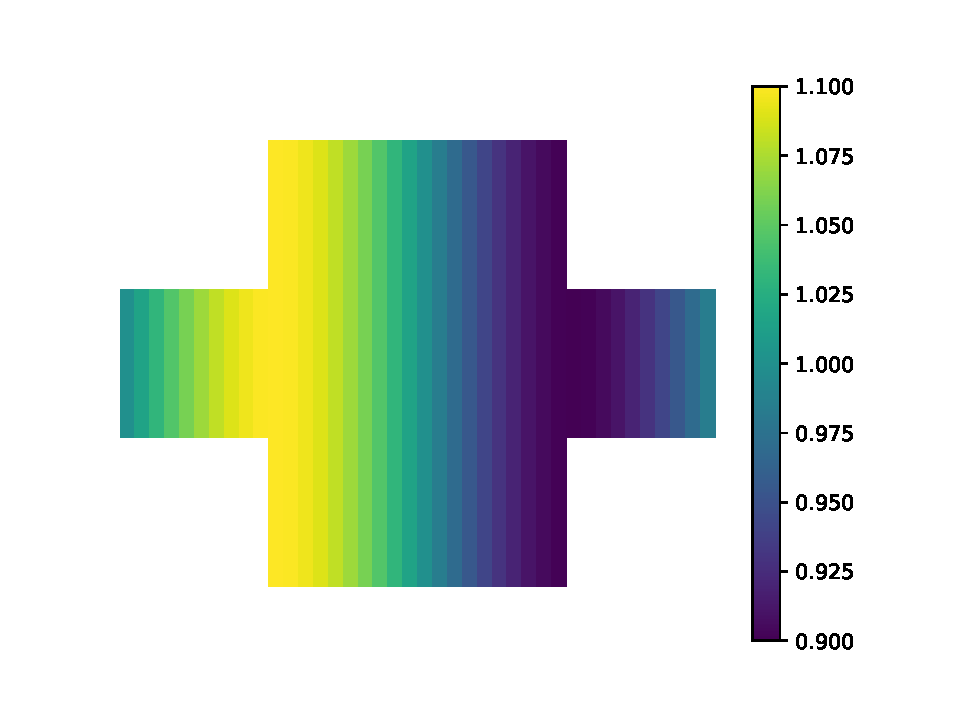
\includegraphics[width=0.7\linewidth]{Figures/std_init_rho.pdf}
	\caption{The figures shows the initial rho in LB units.}
	\label{fig:std_init_rho}
\end{figure} 

\subsection{A standard main file}
\label{sec:a standard main file}
In this section, we describe the main file in \texttt{BADChIMP/src/std\_case}. The code will simulate a standard Navier-Stokes fluid simulation. We are using the BGK-collision routine, as described in the introduction, and we are using the Guo forcing scheme. The geometry and how to generate it is explained in the above section \ref{sec:generating a geometry}. The system has two spatial dimensions and we are using the D2Q9 lattice. The initial density, \texttt{rho}, is defined in the geometry input file, while the initial velocity is set to zero. The system is driven by a body force, \texttt{bodyForce}, and the boundary are of the half-way bounce back type. In the following, a code section is presented first, followed by a more detailed description of its purpose. 
\begin{verbatim}
 10 #include "../LBSOLVER.h"
 11 #include "../IO.h"
 12
 13 // SET THE LATTICE TYPE
 14 #define LT D2Q9
 15
\end{verbatim} 
In line 10, we include the libraries for the classes and functions used in the lattice Boltzmann sections and to read the geometry. In line 11, we include the classes used to read the input file and write the fields to vtk-files. In line 14, we set the lattice type to D2Q9. 
\begin{verbatim}
 16 int main()
 17 {
 18   // *********
 19   // SETUP MPI
 20   // *********
 21   MPI_Init(NULL, NULL);
 22   int nProcs;
 23   MPI_Comm_size(MPI_COMM_WORLD, &nProcs);
 24   int myRank;
 25   MPI_Comm_rank(MPI_COMM_WORLD, &myRank);
 26
\end{verbatim}
Line 16 starts the definition of the main function, and with that the beginning of code block that describes the LB simulations. Lines 21 to 25 initiate MPI's parallel program communication. \texttt{nProcs} holds the total number of processes used in the parallel simulation of the system, and \texttt{myRank} holds the rank of the current processor.
\begin{verbatim}
 27   // ********************************
 28   // SETUP THE INPUT AND OUTPUT PATHS
 29   // ********************************
 30   std::string chimpDir = "BADCHiMP/";
 31   std::string mpiDir = chimpDir + "input/mpi/";
 32   std::string inputDir = chimpDir + "input/";
 33   std::string outputDir = chimpDir + "output/";
\end{verbatim}
Line 30 to 33 set the directory paths used to find input files and where to write the output files. \texttt{chimpDir} is the path to the main code directory. \texttt{mpiDir} is the directory where the python script defining geometry writes its output. This directory needs to match the one given to the \texttt{vtklb}-python object. \texttt{inputDir} is where the input file, read by the \texttt{Input} object, is found. \texttt{outputDir} is where BADChIMP writes its output files.
\begin{verbatim}
 35   // ***********************
 36   // SETUP GRID AND GEOMETRY
 37   // ***********************
 38   Input input(inputDir + "input.dat");
 39   LBvtk<LT> vtklb(mpiDir + "tmp" + std::to_string(myRank) + ".vtklb");
 40   Grid<LT> grid(vtklb);
 41   Nodes<LT> nodes(vtklb, grid);
 42   BndMpi<LT> mpiBoundary(vtklb, nodes, grid);
 43   // Set bulk nodes
 44   std::vector<int> bulkNodes = findBulkNodes(nodes);
\end{verbatim}
In lines 38 and 39, the input-file and the geometry files are read, as described in sections \ref{sec:input} and \ref{sec:lbvtk}.  And, in lines 40 to 42, we define the \texttt{Grid}, \texttt{Nodes}, and \texttt{BndMpi} objects described in sections \ref{sec:grid}, \ref{sec:nodes}, and \ref{sec:bndmpi}, respectively. In line 44, we assign the list of bulk nodes to \texttt{bulkNodes} which contains the nodes numbers that we will loop over in our main-loop. Node types are described in \ref{sec:boundary and bulk nodes}.
\begin{verbatim}
 44   // *************
 45   // READ FROM INPUT
 47   // *************
 48   // Number of iterations
 49   int nIterations = static_cast<int>( input["iterations"]["max"]);
 50   // Write interval
 51   int nItrWrite = static_cast<int>( input["iterations"]["write"]);
 52   // Relaxation time
 53   lbBase_t tau = input["fluid"]["tau"];
 54   // Body force
 55   VectorField<LT> bodyForce(1, 1);
 56   bodyForce.set(0, 0) = inputAsValarray<lbBase_t>(input["fluid"]["bodyforce"]);
\end{verbatim}
In this section, we assign the values given in the input file to variables. The input-file for this case contains four values: three scalars and one vector. The file looks like this:
\begin{verbatim}
<iterations>
  max   5000   # stop simulation after
  write 100    # write interval in steps
<end>
<fluid>
  tau 0.8           # Collision time
  bodyforce 1e-5 0  # Body force
<end>
\end{verbatim}
The file format for input files is described in section \ref{sec:input}. Here, we see that it contains two block, the first one, \texttt{iterations}, sets the number iterations of the write interval. These are set in lines 49 and 51. The second block, \texttt{fluid}, assigns the values that are needed in the LB-method. The collision time is set in line 53 and the body force is set in line 56. Note that for \texttt{bodyForce} we must first define it (line 55) and then use \texttt{VectorField}'s \texttt{set} to assign the value.  
\begin{verbatim}
 59   // ******************
 60   // MACROSCOPIC FIELDS
 61   // ******************
 62   // Density
 63   ScalarField rho(1, grid.size());
 64   // Initiate density from file
 65   vtklb.toAttribute("init_rho");
 66   for (int n=vtklb.beginNodeNo(); n < vtklb.endNodeNo(); ++n) {
 67     rho(0, n) = vtklb.getScalarAttribute<lbBase_t>();
 68   }
\end{verbatim}
Here, we define the fluid density $\rho$ as \texttt{rho} (line 63) and it will have the same number of elements as there are grid nodes. The \texttt{rho} is initialized from the values given in the geometry files. This must be read using the \texttt{vtklb} (in lines 65 to 68). The \texttt{LBvtk} class is described in section \ref{sec:lbvtk}.
\begin{verbatim}
 70   // Velocity
 71   VectorField<LT> vel(1, grid.size());
 72   // Initiate velocity
 73   for (auto nodeNo: bulkNodes) {
 74     for (int d=0; d < LT::nD; ++d)
 75       vel(0, d, nodeNo) = 0.0;
 76   }
\end{verbatim}
The initial velocity is set to zero. The velocity field, $\vec{v}(t, \vec{x})$, is represented by \texttt{vel} (line 71) and is initialized to zeros through the for-loop (line 73-76). 
\begin{verbatim}
 78   // ******************
 79   // SETUP BOUNDARY
 80   // ******************
 81   HalfWayBounceBack<LT> bounceBackBnd(findFluidBndNodes(nodes), nodes, grid);
\end{verbatim}
In line 81, we define object \texttt{bounceBackBnd} that we use for the half-way bounce back boundary conditions. The function \texttt{findFluidBndNodes} returns a list of fluid boundary node number, as defined in section \ref{sec:boundary and bulk nodes}.
\begin{verbatim}
 83   // *********
 84   // LB FIELDS
 85   // *********
 86   LbField<LT> f(1, grid.size()); 
 87   LbField<LT> fTmp(1, grid.size());
 88   // initiate lb distributions
 89   for (auto nodeNo: bulkNodes) {
 90     for (int q = 0; q < LT::nQ; ++q) {
 91       f(0, q, nodeNo) = LT::w[q]*rho(0, nodeNo);
 92     }
 93   }
\end{verbatim}
This section defines and initializes the LB distributions. We define two variables \texttt{f} (line 86) and \texttt{fTmp} (line 87). \texttt{fTmp} is only used as a temporary variable to simplify the propagation step. The initial LB distribution is set, in lines 89 to 93, to $f_q(t=0, \vec{x}) = w_q\rho(\vec{x})$.  
\begin{verbatim}
 95   // **********
 96   // OUTPUT VTK
 97   // **********
 98   auto node_pos = grid.getNodePos(bulkNodes); 
 99   auto global_dimensions = vtklb.getGlobaDimensions();
100   Output output(global_dimensions, outputDir, myRank, 
       nProcs, node_pos);
101   output.add_file("lb_run");
102   VectorField<D3Q19> velIO(1, grid.size());
103   output["lb_run"].add_variable("rho", rho.get_data(), 
       rho.get_field_index(0, bulkNodes), 1);
104   output["lb_run"].add_variable("vel", velIO.get_data(), 
      velIO.get_field_index(0, bulkNodes), 3);
105   outputGeometry("lb_geo", outputDir, myRank, nProcs, nodes, grid, vtklb);
\end{verbatim}
Lines 98 to 105 shows how to add input variables to the \texttt{Output} object \texttt{output}. The plotting has been standardized to work with only 3 dimensional vector fields which is why we have added the \emph{ad hoc} object \texttt{velIO} to help plot the velocity. A new plotting routine has been developed but is not fully tested yet. It will soon be include into the code repository.
\begin{verbatim}
107   // *********
108   // MAIN LOOP
109   // *********
110   for (int i = 0; i <= nIterations; i++) {
\end{verbatim}
This section introduces the beginning of the main time iteration loop. The maximum number of iterations is set by \texttt{nIterations}. 
\begin{verbatim}
111     for (auto nodeNo: bulkNodes) {
112       // Copy of local velocity diestirubtion
113       const std::valarray<lbBase_t> fNode = f(0, nodeNo);
114
115       // Macroscopic values
116       const lbBase_t rhoNode = calcRho<LT>(fNode);
117       const auto velNode = calcVel<LT>(fNode, rhoNode, bodyForce(0, 0));
\end{verbatim}
Here, the loop over all bulk nodes (line 111) is initiated. In this case, this means \emph{all} fluid nodes. \texttt{fNode} holds a copy of the local LB distribution (line 113), and is used repeatedly in this block. The fluid density (\texttt{rhoNode})
\begin{equation*}
\rho = \sum_\alpha f_\alpha,
\end{equation*}   
is calculated in line 116, and the fluid velocity (\texttt{velNode})
\begin{equation*}
u_i = \rho^{-1}\left(\sum_\alpha c_{\alpha i}f_\alpha + \frac{1}{2}F_i\right),
\end{equation*}
is calculated in line 117.
\begin{verbatim}
119       // Save density and velocity for printing
120       rho(0, nodeNo) = rhoNode;
121       vel.set(0, nodeNo) = velNode;
\end{verbatim}
\texttt{rho} and \texttt{vel}, updated in lines 120 and 121, are used for printing the field values to file, and are not strictly necessary for the simulation to run. 
\begin{verbatim}
123       // BGK-collision term
124       const lbBase_t u2 = LT::dot(velNode, velNode);
125       const std::valarray<lbBase_t> cu = LT::cDotAll(velNode);
126       const std::valarray<lbBase_t> omegaBGK 
                              = calcOmegaBGK<LT>(fNode, tau, rhoNode, u2, cu);
\end{verbatim}
This section defines the BGK-collision term. In line 124, we calculate the square of the velocity, $\vec{u}\cdot\vec{u}$, and, in line 125, we calculate the vector object $\vec{c}_\alpha\cdot\vec{u}$. These two variables are used in \texttt{calcOmegaBGK}, the function that calculates the collision term as described in section \ref{sec:macroscopic values and collision}.   
\begin{verbatim}
128       // Calculate the Guo-force correction
129       const lbBase_t uF = LT::dot(velNode, bodyForce(0, 0));
130       const std::valarray<lbBase_t> cF = LT::cDotAll(bodyForce(0, 0));
131       const std::valarray<lbBase_t> deltaOmegaF 
                              = calcDeltaOmegaF<LT>(tau, cu, uF, cF);
\end{verbatim}
This section defines the correction to the BGK-collision term due to the forcing scheme. Besides \texttt{cu}, that is already evaluated, we need to calculate $\vec{u}\cdot\vec{F}$ (line 129) and $\vec{c}_\alpha\cdot\vec{F}$ (line 130). The correction term
\begin{equation*}
	\Delta\Omega_\alpha = \left(1-\frac{1}{2\tau}\right)\left(\frac{\vec{c}_\alpha\cdot\vec{F}}{c_s^2} + \frac{(\vec{c}_\alpha\cdot\vec{F})(\vec{c}_\alpha\cdot\vec{F}) - c_s^2(\vec{u}\cdot\vec{F})}{c_s^4}\right)
\end{equation*} 
is calculated in line 131.
\begin{verbatim}
133       // Collision and propagation
134       fTmp.propagateTo(0, nodeNo, fNode + omegaBGK + deltaOmegaF, grid);
135
136     } // End nodes
137
138     // Swap data_ from fTmp to f;
139     f.swapData(fTmp);  // LBfield
\end{verbatim}
In the last line of the bulk-node loop block, we will propagate the LB distribution in \texttt{f} to the LB distribution \texttt{fTmp} using the \texttt{LbField} function \texttt{propagateTo}, described in section \ref{sec:field classes}. Line 136 ends the bulk-node for-loop block. To finish the propagation scheme \texttt{f} and \texttt{fTmp} swaps data on line 139 so that we can still use \texttt{f} as our lb distribution when we use boundary condition objects and functions.
\begin{verbatim}
141     // *******************
142     // BOUNDARY CONDITIONS
143     // *******************
144     // Mpi
145     mpiBoundary.communicateLbField(0, f, grid);
146     // Half way bounce back
147     bounceBackBnd.apply(f, grid);
\end{verbatim}
After we have finished with the bulk nodes, we apply the boundary conditions. In line 145, we communicate with neighboring processes, as part of the parallelization scheme. The communication is handled by the \texttt{mpiBoundary} object (see section \ref{sec:bndmpi} for more details). The bounce back boundary scheme is conducted in line 147 with \texttt{bounceBackBnd}'s \texttt{apply} function.
\begin{verbatim}
149 // *************
150 // WRITE TO FILE
151 // *************
152     if ( ((i % nItrWrite) == 0)  ) {
153       for (auto nn: bulkNodes) {
154         velIO(0, 0, nn) = vel(0, 0, nn);
155         velIO(0, 1, nn) = vel(0, 1, nn);
156         velIO(0, 2, nn) = 0;
157       }
158       output.write("lb_run", i);
159       if (myRank==0) {
160         std::cout << "PLOT AT ITERATION : " << i << std::endl;
161       }
162     }
\end{verbatim}
\begin{figure}[h]
	%	\centering
	\begin{subfigure}{0.40\textwidth}
		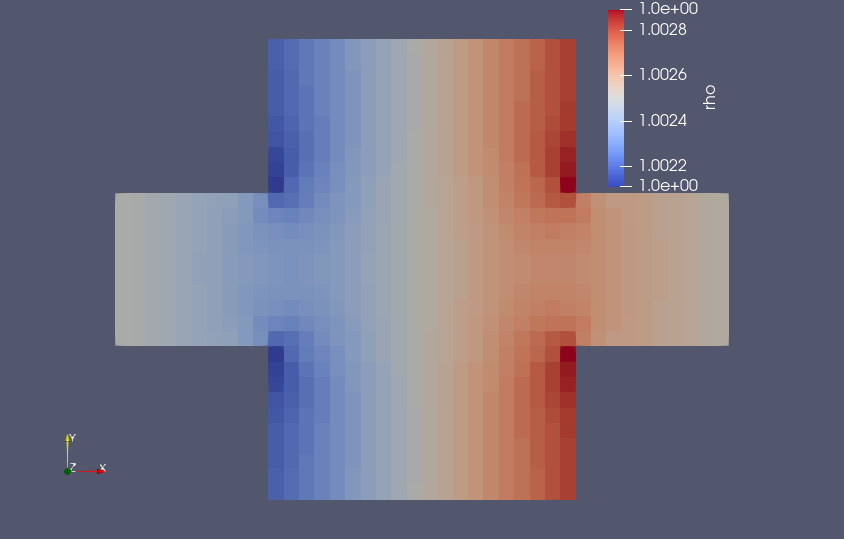
\includegraphics[width=1.2\textwidth]{./Figures/std_case_run_rho.png}
		\caption{Density}
	\end{subfigure}
	\begin{subfigure}{0.40\textwidth}
		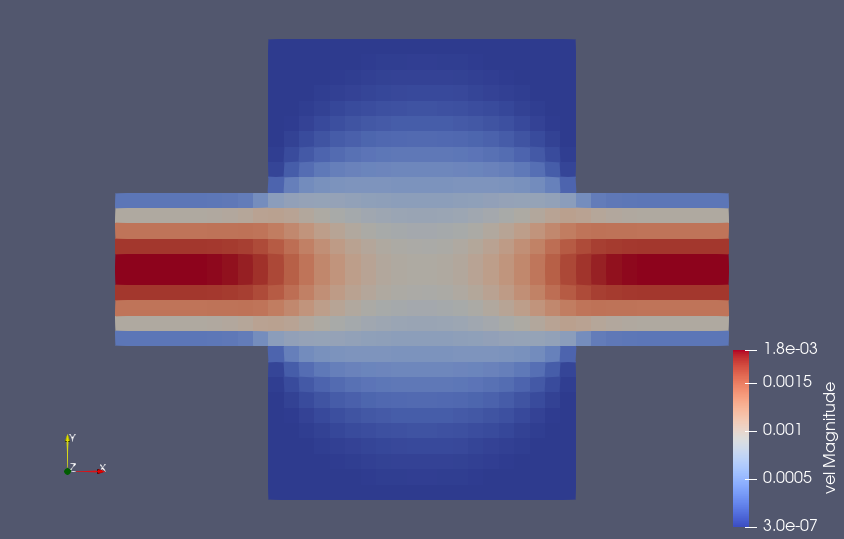
\includegraphics[width=1.2\textwidth]{./Figures/std_case_run_vel.png}
		\caption{Velocity magnitude}
	\end{subfigure}	
	\caption{The figures shows the fluid density in (a) and the velocity magnitude, $\sqrt{\vec{u}\cdot\vec{u}}$, in (b) for the run described in this section. All values are given in LB units.}
	\label{fig:std_case rho vel}
\end{figure}   All field added to the \texttt{output} object is plotted by using the \texttt{write} command in line 158. In line 153 to 157 we updated the values in the \emph{ad hoc} velocity object \texttt{velIO}.
\begin{verbatim}
164   } // End iterations
165
166   MPI_Finalize();
167
168   return 0;
169 }
\end{verbatim}
Finally, we are at the end of the main-file. The time-iteration loop block ends at line 164. The MPI communication is shut down with \texttt{MPI\_Finalize} and line 168 and 169 ends the main function.

After the program has finished, all files written by the \texttt{Output} objects will be found in the folder set by \texttt{outputDir} in line 33. These files are in the vtk format, and in this project we have used paraview\footnote{see https://www.paraview.org/} to view and analyze the files.  In figure xx we show the density and velocity magnitude for a run of the case above using the paraview program.
 

\chapter{Simulation of non-Newtonian rheologies}
\label{sec:simulation of non-Newtonian rheologies}
In many fluids the relation between the viscous stress and the velocity changes can be extremely non-
linear, and it may very well depend on other properties of the fluid. These fluids are called non-Newtonian fluids. A subset of these, where ${\sigma'_{i j} = 2\mu_\mathrm{eff}(\dot{\gamma}) E_{ij}}$, are classified as generalized Newtonian fluid. Here, the viscosity is a function of the strain rate ${\dot{\gamma}=\sqrt{2E_{ij}E_{ij}}}$.

For a Carreau-model fluid
\begin{align}
\sigma'_{i j} = 2\bigg\{\mu_\infty + \left(\mu_0 -\mu_\infty\right)\big[1 + (\lambda \dot{\gamma})^{y_0} \big]^{\frac{n-1}{y_0}} \bigg\} E_{ij}
= 2\mu_\mathrm{eff} E_{ij} \, ,\label{eq:carreau}
\end{align}
where $\mu_0$ is the viscosity at zero strain rate, $\mu_\infty$ is the viscosity at infinite strain rate, $\lambda$ is the time constant that determines the onset of shear thinning, $y_0$ is a tuning parameter used
to improve the viscosity match at shear rates ${\dot{\gamma}/\lambda}\sim 1$ (here, ${y_0 = 2}$), and $n$ is the shear thinning index. This index is known to depend on the
polymer concentration. the relaxation time $\lambda$ normally decreases by decreasing the intrinsic viscosity. 

For a Papanastasiou-model type fluid \cite{papanastasiou1987flows}
\begin{align}
\sigma'_{i j} = 2\Bigg\{\mu_p + \frac{\tau_0 \left[1-\exp\left(-m \sqrt{2E_{ij}E_{ij}}\right)\right]}{2\sqrt{2E_{ij}E_{ij}}} \Bigg\} E_{ij} = 2\mu_\mathrm{eff} E_{ij} \, ,
\end{align}
where $\mu_p$ is the plastic viscosity of the yielded material, and $\tau_0$ is yield stress.

For a Papanastasiou-model type Herschel-Bulkley fluid
\begin{align}
\sigma'_{i j} = 2\Bigg\{\mu_p \left(2E_{ij}E_{ij}\right)^{(n-1)/2} + \frac{\tau_0 \left[1-\exp\left(-m \sqrt{2E_{ij}E_{ij}}\right)\right]}{2\sqrt{2E_{ij}E_{ij}}} \Bigg\} E_{ij} = 2\mu_\mathrm{eff} E_{ij} \, ,
\end{align}



\section{Calculating the effective LB relaxation time $\tau$ for non-Newtonian rhelogies}
In the LB model, it may be shown that the strain rate tensor
\begin{align}
E_{ij} = \frac{1}{2 \rho c^2_\mathrm{s} \tau \Delta t}\widetilde{E}_{ij},\label{eq:Etilde1}
%\left[\sum_\alpha f_\alpha^\mathrm{neq} c_{\alpha i} c_{\alpha j} + \frac{1}{2} \big(u_iF_j+u_jF_i + u_i u_j q + c^2_\mathrm{s} q \delta_{ij}\big)\Delta t\right],
\end{align}
where ${f_\alpha^\mathrm{neq}\equiv f_\alpha - f_\alpha^\mathrm{eq}}$ and
\begin{align}
\widetilde{E}_{ij} &= -\left[\sum_\alpha f_\alpha^\mathrm{neq} c_{\alpha i} c_{\alpha j} + \frac{1}{2} \big(u_iF_j+u_jF_i + u_i u_j q + c^2_\mathrm{s} q \delta_{ij}\big)\Delta t\right] \notag\\
&= -\left[\sum_\alpha f_\alpha^\mathrm{neq} Q_{\alpha ij} + \frac{1}{2} \big(u_iF_j+u_jF_i + u_i u_j q \big)\Delta t\right]\label{eq:Etilde2}
\end{align}

\begin{align}
\tau = \frac{1}{\rho c^2_\mathrm{s} \Delta t}\mu_\mathrm{eff}\Big(\widetilde{E}_{ij}\widetilde{E}_{ij}\Big)+\frac{1}{2},
\end{align}
where $\mu_\mathrm{eff}$ may be tabulated as a function of the contraction of $\widetilde{E}_{ij}$.

\section{Running a non-Newtonian flow simulation}
To run a simulation of a fluid exhibiting non-Newtonian rheology, the simulator needs the viscosity as a function of the contraction $\widetilde{E}_{ij}\widetilde{E}_{ij}$, where $\widetilde{E}_{ij}$ is defined in Eqs.~\eqref{eq:Etilde1} and \eqref{eq:Etilde2}. This is done through a file containing the tabulated viscosity values with corresponding values for $\widetilde{E}_{ij}\widetilde{E}_{ij}$. This file may generated using a Python script found in the \texttt{PythonScripts} folder found in the code root directory.

\subsection{Python script for generating a tabulated viscosity file} \label{subsec:py_visc}

The python script \texttt{viscosity\_tabulationDEMO.py} shows an example of how the file containing viscosity values may be generated. Here, the Carreau rheology model (see Eq.~\eqref{eq:carreau}) is chosen as a demonstration. The Carreau model takes 5 input parameters: $\mu_\infty$, $\mu_0$, $\lambda$, $y_0$, and $n$ (see Eq.~\eqref{eq:carreau} for definitions). In the Python script, these parameters must be given in lattice Boltzmann units. Given these parameters, the script generates a file \texttt{test\_rheo.dat}. The first line of this file contains the length of table. The rest of the file is divided into 2 columns: the first column contains values of $\widetilde{E}_{ij}\widetilde{E}_{ij}$, while the second column contains the corresponding effective dynamic viscosities $\mu_\mathrm{eff}$. In figure \ref{fig:carreau plot} we show the generated viscosity that we will use in the test run in this section.
\begin{figure}
	\centering
	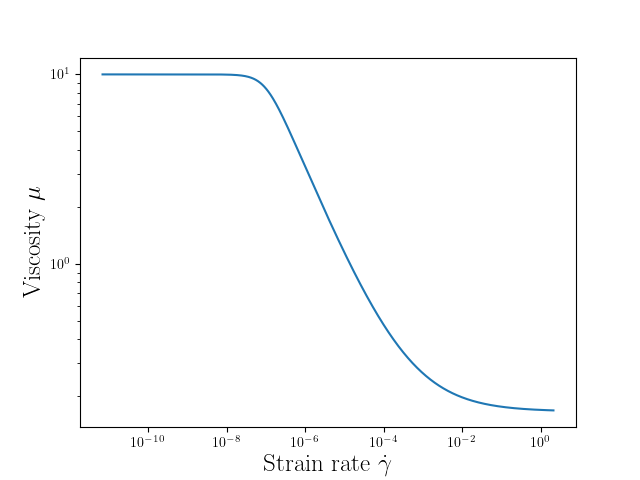
\includegraphics[width=0.7\linewidth]{Figures/carreau_plot.png}
	\caption{Figure of the tabulated viscosity as a function of strain rate, $\dot{\gamma} = \sqrt{2E_{ij}E_{ij}}$.}
	\label{fig:carreau plot}
\end{figure} 

\subsection{Key features in the main-file}
\subsubsection{Initializing chosen rheology}
Following the directions given in section~\ref{subsec:py_visc} for generating an file containing a tabulated viscosity behavior, one needs to facilitate the non-Newtonian flow behavior in the BADChIMP simulator. The first step is to import the viscosity property by constructing a \texttt{GeneralizedNewtonian} object in when setting up the grid and geometry.   
\begin{verbatim}
// ********************************
// SETUP THE INPUT AND OUTPUT PATHS
// ********************************
std::string chimpDir = "/BADChIMP/";
...
std::string inputDir = chimpDir + "input/";
...
// ***********************
// SETUP GRID AND GEOMETRY
// ***********************
...
// Read rheology
GeneralizedNewtonian<LT> carreau(inputDir + "test.dat");
\end{verbatim}
In our example we have chosen the object name \texttt{carreau}. In the initialization step above, it takes the \texttt{test.dat} file as input. This file, which can be generated by following the directions given in section~\ref{subsec:py_visc}, must be located in the directory \texttt{inputDir}.
\begin{figure}[!h]
	%	\centering
	\begin{subfigure}{0.30\textwidth}
		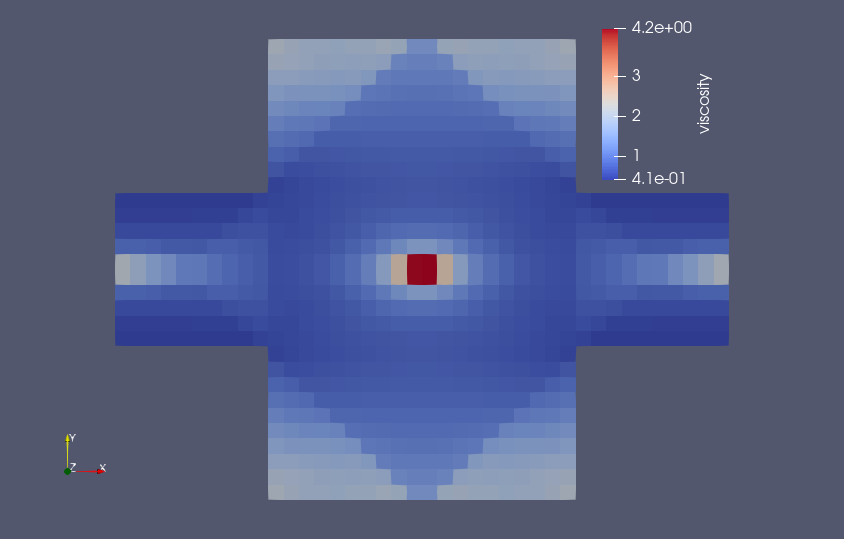
\includegraphics[width=1.2\textwidth]{./Figures/polymer_run_viscosity.png}
		\caption{Viscosity}
	\end{subfigure}
	\begin{subfigure}{0.30\textwidth}
		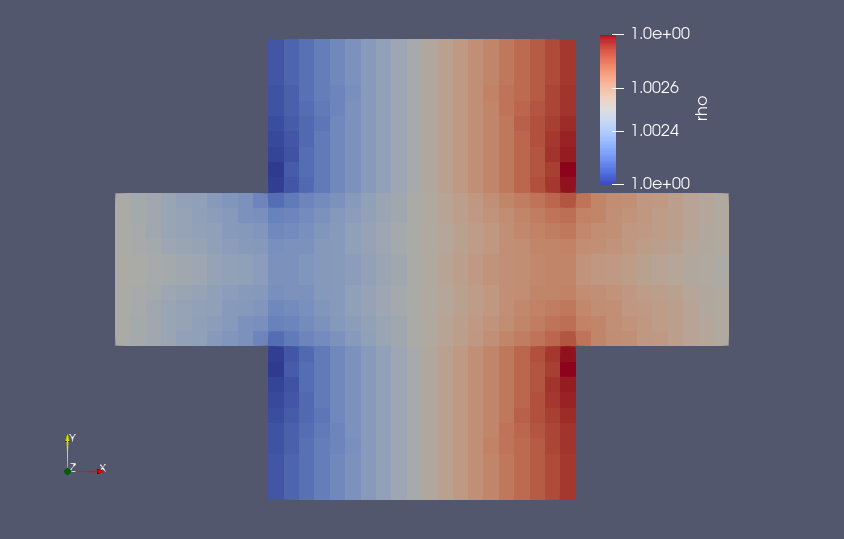
\includegraphics[width=1.2\textwidth]{./Figures/polymer_run_rho.png}
		\caption{Density}
	\end{subfigure}
	\begin{subfigure}{0.30\textwidth}
		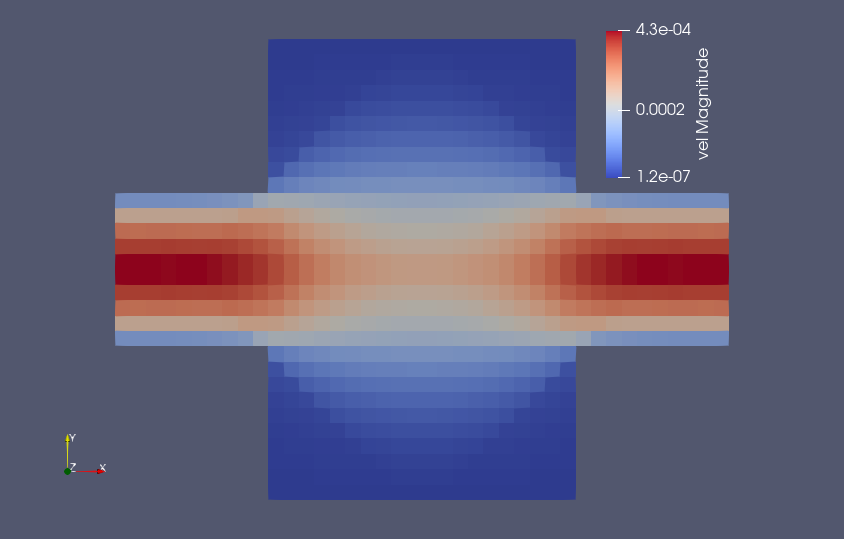
\includegraphics[width=1.2\textwidth]{./Figures/polymer_run_vel.png}
		\caption{Velocity magnitude}
	\end{subfigure}	
	\caption{The figures shows the viscosity in (a), the fluid density in (b) and the velocity magnitude, $\sqrt{\vec{u}\cdot\vec{u}}$, in (c) for the run described in this section. All values are given in LB units.}
	\label{fig:polymer rho vel}
\end{figure}

The non-Newtonian behavior is included in the main time loop through the the BGK collision term \texttt{omegaBGK} and, through the modified relaxation time \texttt{tau}, the force term \texttt{deltaOmegaF}.
\begin{verbatim}
// *********
// MAIN LOOP
// *********
...
auto omegaBGK = carreau.omegaBGK(fNode, rhoNode, velNode, u2, cu,
                                   bodyForce(0, 0), 0);
...
tau = carreau.tau();
viscosity(0, nodeNo) = carreau.viscosity();
const std::valarray<lbBase_t> deltaOmegaF = calcDeltaOmegaF<LT>(tau, cu, uF, cF);
\end{verbatim}
Note that \texttt{carreau.omegaBGK()} must be called ahead of \texttt{carreau.tau()} in order to get the updated value of \texttt{tau}. We can also get the viscosity by using \texttt{GeneralizedNewtonian}'s \texttt{viscosity} function. The code snippets above is copied from the main-file in folder \texttt{/src/polymer\_viscosity\_tabulation}.
    

In figure \ref{fig:polymer rho vel} we show the viscosity, density and velocity magnitude for a Carreau rehology. The geometry and the body force is equal to the standard case presented in section \ref{sec:a standard main file}.

\chapter{Future work/plans} 

Our main plan for the numerical package developed in this project is that we aim to include all new LB methods developed in future projects into the BADChIMP code repository, so that it will become available for all users. Hopefully, this will also keep the development of the core libraries up to speed with new developments in both hardware and software, so that the code will evolve and improve as a general tool for scientific computations.    

The code and user manual will continuously be improved as stated in the introduction. It is our intention that new methods and features will be added as their own chapters, so that the core of this manuscript will stay more or less the same. 

The first planned extension of the code is to include more general polymer models like the C-Fene-P model. Numerical methods are currently being developed by PhD student Bjarte Hetland, as part of his thesis work, and will be include in the BADChIMP code when finished. 

The lattice Boltzmann code is also used in projects on bio-cementation, turbulent flow simulations for wind turbine modeling, and three phase systems, water, oil, and CO$_2$, for the study of CO$_2$ storage in old oil reservoirs. We expect that the algorithms developed in these project will become part of the BADChIMP code.   

On a more code specific level, we also plan to improve our geometry input scheme so that we could add vector and tensor fields as input. We would also like to add attributes to a small subsets of nodes to reduce the size of input files.  


\appendix


\chapter{Parallelization}\label{sec:parallelization}

\section{Deadlock prevention}
In the LB code each processor has a list of neighboring processors which it sends and receives data from. This list has the following properties:
\begin{enumerate}
	\item If processor A is in processor B's list of neighbors, then processor B will be in
	processor A's list of neighbors.
	\item Processor A is not part of its own list of neighbors.
	\item A list of neighbors is sorted in ascending order, based on rank.
\end{enumerate}
The send/receive code follows the structure given below:
\begin{verbatim}
    for (auto neigRank: listOfNeighbors) {
        if (myRank < neigRank) {
            // SEND DATA to neigRank
            // RECEIVE DATA from neigRank
            } else {
            // RECEIVE DATA from neigRank
            // SEND DATA to neigRank
        }
    }
\end{verbatim}
We will argue, based  on the Coffman conditions\footnote{See: https://en.wikipedia.org/wiki/Deadlock}, that this structure is enough to avoid \emph{deadlock}. 

Here, we will show that the assumption of a \emph{circular wait condition} will lead to a contradiction. We assume that there are $n$ processes (or processors), $p$, waiting for each other, so that $p_0$ is waiting for $p_1$, $p_1$ is waiting for $p_2$, and so on until $p_{n-1}$ is waiting for $p_0$. We call the set of processes that are part of the circular wait loop for a circular wait-set (CWS). Now, let $p_k$ be the process with the lowest rank in a CWS. Since it has the lowest rank, it must be waiting to send to a process, $p_{k+1}$, with a higher rank, as given by the code structure above. And, since $p_{k+1}$ is in $p_k$'s list of neighbors, $p_k$ is in $p_{k+1}$'s list of neighbors. $p_{k+1}$ must either be waiting to send to, or receive from, $p_{k+2}$. If $p_{k+2}$ is equal to $p_k$ we know that $p_k$'s rank is lower than $p_{k+1}$'s and $p_{k+1}$ should be waiting to receive data from $p_k$. But this makes the \emph{circular wait condition} stated above invalid. Hence, $p_{k+2}$ must be a different process than $p_k$. We then know, by assumption, that the rank of $p_{k+2}$ is higher than $p_k$'s, which means it is in a later position in $p_{k+1}$'s list of neighbors (since it was sorted in ascending order). $p_{k+1}$ should then already have been waiting to receive data from $p_k$, as the list of neighbors is traversed from lowest to highest values. But since $p_k$ is already waiting to send to $p_{k+1}$, this will again make the \emph{circular wait condition} false, as $p_k$ would no longer wait to send to $p_{k+1}$. Thus, the assumption of a \emph{circular wait} condition leads to a contraction, which proves, by \emph{reductio ad absurdum}, that the proposed parallel communication protocol cannot lead to a \emph{deadlock} situation.

\chapter{Geometry file format}\label{sec:geometry file format}
This is a description of the geometry file format we have called \emph{vtklb}. This is the format that is read by BADChIMP to include geometries and spatial varying data. This formate is based on the VTK-file format\footnote{https://vtk.org/wp-content/uploads/2015/04/file-formats.pdf}.

The overall tile format is given below.
\begin{verbatim}
# BADChIMP vtklb Version 0.1     <header>
one line descriptioin            <title> 
ASCII | BINARY                   <data type>
DATASET type                     <geometry/topology>
...
POINT_DATA n                     <dataset attributes>
...
\end{verbatim}
\section{Geometry/topology}
The available dataset-type for geometry/topology is the "unstructured lb grid" and "structured lb grid":
\begin{verbatim}
DATASET UNSTRUCTURED_LB_GRID
NUM_DIMENSIONS nd               <nd: int number of spatial dimension>
GLOBAL_DIMENSIONS n0 n1 ...     <Size of the bounding box of the system>
USE_ZERO_GHOST_NODE             <use node 0 as the default ghost node>
POINTS n dataType               <n: number of points>
p1_xp1_y...                     <point/node spatial position>
p2_xp2_y...
...
LATTICE nq dataType             <nq: number of basis vectors>
c0_xc0_y...                     <basis vecotor elements>
c1_xc1_y...
...
NEIGHBORS dataType              <list of neighbor nodes for each node>
i1_0i1_1...i1_(nq-1)            <node number of neighbor nodes>
i2_0i2_1...i2_(nq-1)
...
in_0in_1...in_(nq-1)
PARALLEL_COMPUTING rank         <rank: rank of the current processor>
PROCESSOR n rank                <n: number of point, rank: neighbor processor>
i0j0                            <i: node this rank, j: node neighbor rank>
i1j1
...
i(n-1)j(n-1)
\end{verbatim} 
Comments to entries:
\begin{description}
\item[\texttt{dataType}:] Numrical type of entry data, i.e. \texttt{int} (integer) , \texttt{float} (float), \texttt{double} (double), ... 
%	
\item[\texttt{NUM{\_}DIMENSIONS}:] (Optional, Default: nd=3)  Specify number of spatial dimensions. In vtk it seems that all vectors and positions are given with three components. 
%
\item[\texttt{GLOBAL{\_}DIMENSIONS}:] Gives the size of the system in each Cartesian direction include the ghost node rim. This entry should be the same for all processors. This information is needed by the vtk-output routine.
%
\item[\texttt{USE{\_}ZERO{\_}GHOST{\_}NODE}:] (Optional) Treat node 0 as a placeholder for a node that is not in use (i.e solid nodes). This means that we begin numbering points from 1, \emph{not} 0. If the key word is written then this feature is enabled.
%
\item[\texttt{POINT}:] Same as for the vtk-format. NB if \texttt{USE{\_}ZERO{\_}GHOST{\_}NODE} is enabled then the the first entry has node number 1, the next has 2 and so on. If \texttt{USE{\_}ZERO{\_}GHOST{\_}NODE} is disabled  the first entry has node number 0.
%
\item[\texttt{LATTICE}:] Description of the set of basis vector. We can check these with the ones used in the BADChIMP code and map one set to the other if that is needed.
%
\item[\texttt{NEIGHBORS}:]  For each node there is a list of \texttt{nq} nodes. The node number corresponds to the position in the list under the \texttt{POINTS}-keyword and the position in the list of neighbors corresponds to the basic vector in the list under the \texttt{LATTICE}-keyword.
%
\item[\texttt{PARALLEL{\_}COMPUTING}:] Begins the block describing the processor-to-processor communication. \texttt{rank} is the rank of the current processor.
%
\item[\texttt{PROCESSOR}:]  Information about neighboring processor. \texttt{n} is the number of nodes at the current processor that is used to represent the nodes at a neighboring process. \texttt{rank} is the rank of the neighboring node. In the list under the keyword, the first entry, \texttt{i}, is the node number in the geometry in the current processor that represent the node with number \texttt{j} in the neighboring rank, which is the second entry on the line.
\end{description}


\begin{verbatim}
DATASET STRUCTURED_LB_GRID
NUM_DIMENSIONS nd               <nd: int number of spatial dimension>
GLOBAL_DIMENSIONS n0 n1 ...     <Size of the bounding box of the system>
LOCAL_DIMENSIONS n0 n1 ...      <Size of the system on the given processor 
                                 excluding the rim of ghost nodes>
LOCAL_RIM_WIDTH nw              <nw: int number of rim width>
LOCAL_TO_GLOBAL_POS po p1 ...   <Sets the global position relative to 
                                 the local origo>
LATTICE nq dataType             <nq: number of basis vectors>
c0_xc0_y...                     <basis vecotor elements>
c1_xc1_y...
...
PERIODIC_NODES n rank           <n: number of point, rank: neighbor processor>
i0j0                            <i: 'ghost' node, j: bulk node> 
i1j1 
...
PARALLEL_COMPUTING rank         <rank: rank of the current processor>
PROCESSOR n rank                <n: number of point, rank: neighbor processor>
i0j0                            <i: node this rank, j: node neighbor rank>
i1j1
...
i(n-1)j(n-1)
\end{verbatim}
Additional comments to entries:
\begin{description}
\item[\texttt{PERIODIC{\_}NODES}:] Sets the nodes that are periodic on one given processor. This needs to be handled separately.	
\end{description}	
	
\section{Dataset attributes}
Here we use the same formalism as the vtk-file format using the keywords, e.g., \texttt{SCALARS} and \texttt{VECTORS}. This information is written after the \texttt{POINT{\_}DATA}-keyword.
\begin{verbatim}
POINT_DATA n                     <n: number of point>
SCALARS dataName dataType        <list of scalar values>
s0                               <s: scalar numerical value of type dataType>
s1
...
s(n-1)
\end{verbatim}

\section{Example of node numbering}
\begin{figure}[h]
	\begin{subfigure}{0.32\textwidth}
		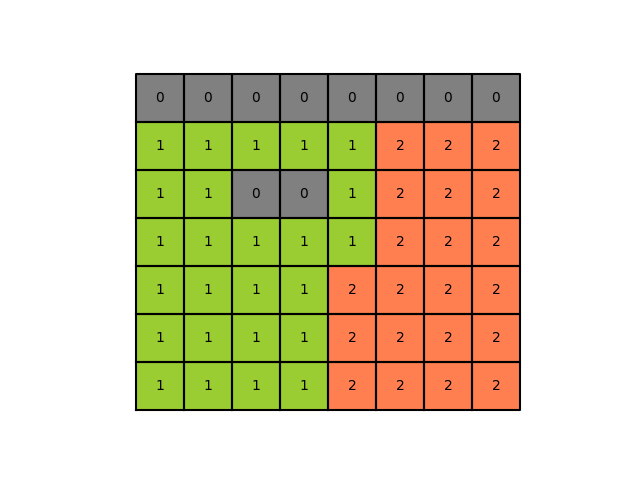
\includegraphics[width=1.2\textwidth]{./Figures/geo_plot01.png}
	\end{subfigure}
	\begin{subfigure}{0.32\textwidth}
	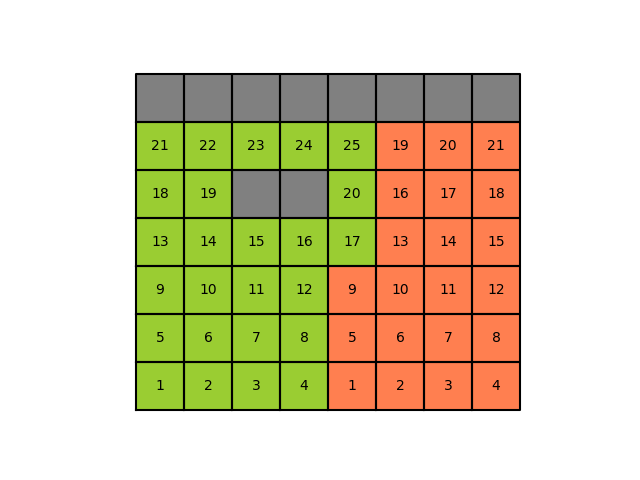
\includegraphics[width=1.2\textwidth]{./Figures/geo_plot02.png}
    \end{subfigure}
	\begin{subfigure}{0.32\textwidth}
	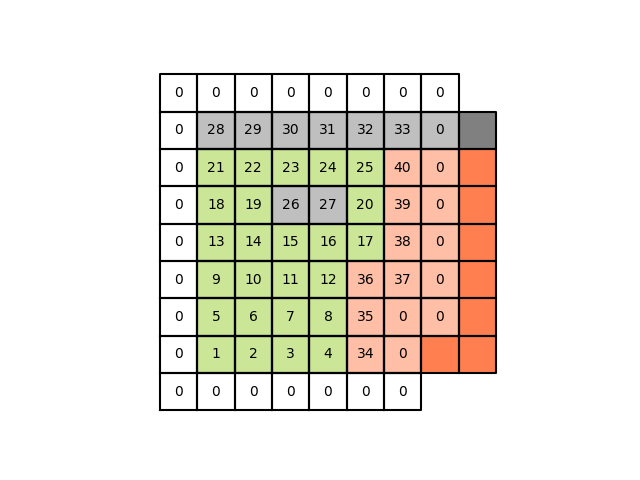
\includegraphics[width=1.2\textwidth]{./Figures/geo_plot03.png}
    \end{subfigure}
	\caption{Concept figure for the node numbering scheme used in BADChIMP. Left: Geometry where 0 is solid, 1 shows nodes on processor with rank 0, and 2 shows nodes on processor with rank 1. Middle: Shows the local node labels on the two processors. Right: Local labeling for processor 1 with rank 0.}\label{fig:geo_plot}
\end{figure}

Figure \ref{fig:geo_plot} (left) shows an example geometry, where the green and orange areas shows the partitioning of the computational nodes between processor 1 and 2. In each processor, the fluid nodes are consecutively labeled starting from 1. 

Figure \ref{fig:geo_plot} (middle) shows labeling of the fluid nodes, where the solid nodes (in gray) will not be given global labels.  
For standard fluid flow simulations we would like to allocate memory for the solid wall nodes, but we do not need to transfer wall values between processors. 

Figure \ref{fig:geo_plot} (right) shows the local labeling for processor 1. Here, the labeling of the fluid nodes follow that of the fluid nodes on processor 1 illustrated in the middle figure. Note, however, that the fluid nodes that belongs to the neighboring  processor are relabeled. These nodes need to be linked to the local labels on processor 2. The zero label is used as a default ghost node.

\renewcommand\bibname{References}
\bibliographystyle{plain}
\bibliography{references} 	
 	
\end{document}